\documentclass[12pt,english,pdflatex]{aghdpl}
%%%%%%%%%%%%%%%%%%%%%%%%%%%%%%%%%%%%%%%%%%%%%%%%%%%%%%%%%%%%%%%%%%%%%%
%%% Packages added by ali
\usepackage{latexsym}
\usepackage{amssymb}
\usepackage{amsmath}
\usepackage{amsfonts}
\usepackage{times}
\usepackage{anysize,url,color,graphicx}%times
\usepackage{tikz}
\usepackage{tabularx}
%%%%% Some commands:
\newcommand{\tbc}[1]{\colorbox{blue}{(#1)}} % to be considered
\newcommand{\example}[1]{\colorbox{green}{(#1)}}
\newcommand{\todosm}[1]{\colorbox{yellow}{(#1)}}
\newcommand{\todoali}[1]{\colorbox{magenta}{(#1)}}
\newcommand{\fixme}[1]{\colorbox{yellow}{FIXME: (#1)}}
\newcommand{\redbox}[1]{\colorbox{red}{ #1 }}
\newcommand{\cyanbox}[1]{\colorbox{cyan}{ #1 }}
\newcommand{\greenbox}[1]{\colorbox{green}{ (#1)}}
\newcommand{\bluebox}[1]{\colorbox{blue}{ (#1)}}
\newcommand{\magentabox}[1]{\colorbox{magenta}{ (#1)}}
%%%%% Some colors:
\newcommand{\lst}[1]{\lstinline{#1}}
\newcommand{\al}[1]{{\color{red}{#1}}}
\newcommand{\cb}[1]{{\color{blue}{#1}}}
\newcommand{\cm}[1]{{\color{magenta}{#1}}}
\newcommand{\cy}[1]{{\color{yellow}{#1}}}
\newcommand{\cg}[1]{{\color{green}{#1}}}
%%%%% Definitions
\newtheorem{Def}{Definition}
\newtheorem{The}{Theorem}
\newtheorem{Lem}{Lemma}
\newtheorem{Ax}{Axiom}
\newtheorem{Cor}{Corrolary}
%%%%% Dimensions if necessary:
%\textwidth 16cm
%\textheight 22cm
\parskip 3mm
\parindent 20mm
%\topmargin -1mm
%\evensidemargin -3mm
%\oddsidemargin -3mm
%\marginsize{23mm}{20mm}{15mm}{15mm}
%\graphicspath{{./PICTURES/}}
\renewcommand{\baselinestretch}{1.0}
\sloppy
%%%%% End by ali
%%%%%%%%%%%%%%%%%%%%%%%%%%%%%%%%%%%%%%%%%%%%%%%%%%%%%%%%%%%%%%%%%%%%%%
\usepackage[T1]{fontenc}
\usepackage[utf8]{inputenc}
\usepackage{color}
\usepackage{babel}
\usepackage{array}
\usepackage{float}
\usepackage{textcomp}
\usepackage{setspace}
\usepackage{subscript}
\onehalfspacing
\usepackage[unicode=true,
 bookmarks=true,bookmarksnumbered=true,bookmarksopen=true,bookmarksopenlevel=2,
 breaklinks=true,pdfborder={0 0 0},pdfborderstyle={},backref=false,colorlinks=true]
 {hyperref}
\hypersetup{pdftitle={dyplom},
 pdfauthor={Imie Nazwisko},
 pdfsubject={Temat},
 pdfkeywords={słowa kluczowe},
 urlcolor=blue}

\makeatletter

%%%%%%%%%%%%%%%%%%%%%%%%%%%%%% LyX specific LaTeX commands.
%% Because html converters don't know tabularnewline
\providecommand{\tabularnewline}{\\}

%%%%%%%%%%%%%%%%%%%%%%%%%%%%%% User specified LaTeX commands.
% dodatkowe pakiety
\usepackage{enumerate}
\usepackage{listings}
% Numeracja po kolei rysunkow, tabel i wzorow
\usepackage{chngcntr}
\counterwithout{figure}{chapter}
\counterwithout{table}{chapter}
\counterwithout{equation}{chapter}
%
\lstloadlanguages{TeX}
\usepackage{caption} 
\captionsetup[figure]{labelformat=simple, labelsep=period}
\captionsetup[table]{labelformat=simple, labelsep=period}
\captionsetup[algorithm]{labelformat=simple, labelsep=period}
%\captionsetup{font=small}
\captionsetup{margin=10pt, font={small}, labelfont=bf, format=hang}
\usepackage{esint}
\clubpenalty = 10000
\widowpenalty = 10000
%\usepackage{graphicx}
%\usepackage{grfext}
%\AtBeginDocument{%
% \PrependGraphicsExtensions*{
%    .mps,.MPS,.pdf,.PDF,.eps,.EPS,.ps,.PS,
%    .png,.PNG,.jpg,.jpeg,.JPG,.JPEG,
%    .funny,.foobar
%  }%
%  \PrintGraphicsExtensions % see .log file
%}
% \usepackage[style=numeric-comp]{biblatex}
% \setlength{\itemsep}{-1\parsep}
%---------------------------------------------------------------------------
%\usepackage{epstopdf}

%\@ifundefined{showcaptionsetup}{}{%
% \PassOptionsToPackage{caption=false}{subfig}}
\usepackage{subfig}

\usepackage{listings}

\definecolor{deepblue}{rgb}{0,0,0.5}
\definecolor{deepred}{rgb}{0.6,0,0}
\definecolor{deepgreen}{rgb}{0,0.5,0}
% I am far from expert in decorations/view-planning.
% Any ideas with listings appreciated.
\lstset{language={Python},
alsolanguage={bash},
breaklines=true,
otherkeywords={self, True, False, None},
keywordstyle=\color{deepblue},
emphstyle=\color{deepred},
stringstyle=\color{deepgreen},
fontadjust=true,
numberstyle={\tiny},
stepnumber=1,
tabsize=4,
numbersep={-7pt},
numbers=right,
numberstyle={\tiny},
backgroundcolor={\color{cream}}}

\makeatother

\begin{document}
\sffamily  %%%%% Font suggested by ali
\author{Sebastian Morawiec}
\shortauthor{S. Morawiec}
\titlePL{Design and Implementation of an Experimental SAT Solver}
\titleEN{Projekt i implementacja eksperymentalnego solvera SAT}
\shorttitle{Design and Implementation of an Experimental SAT Solver}
\faculty{Wydział Elektrotechniki, Automatyki,\\Informatyki i Inżynierii Biomedycznej}
\division{Katedra Automatyki i Inżynierii Biomedycznej}
\specialization{Automatyka i Robotyka}
\thesistype{Praca dyplomowa magisterska}
\supervisor{Prof. dr hab. inż. Antoni Ligęza}
\acknowledgements{\textit{I would first like to thanks my advisor, Professor Antoni
Ligęza, for his patience, knowledge and support.
I would also like to express my gratitude to my closest family and my fiancée,
for providing me with continuous support and encouragement throughout
my years of study and through the process of  writing this MSc thesis.}}
\titlepages
\setcounter{tocdepth}{2}

\tableofcontents{}

\chapter{Introduction}
\label{chap:Wstep}

\section{Brief History of SAT and Logic}
\label{sec:intro_SAT}

The history of mathematical logic, as we know it today, started with
publication of \textit{The Mathematical Analysis of Logic} in 1847 \cite{boole1847mathematical} .
Of course -- before that happened, the idea of logic and some logical systems had been
developed -- the most famous example being \textit{Term Logic} assigned to well
known ancient Greek philosopher - Aristotle\footnote{\url{www.britannica.com/topic/history-of-logic} for more information}.
However, it was George
Boole with previously mentioned work \cite{boole1847mathematical}, who created an idea of algebraic
structures that were later developed by William Jevons in \textit{Pure
Logic, or the Logic of quality apart from quantity} \cite{jevons2015pure} work published
in 1863. Nowadays those structures are known as \textit{Boolean Algebra}, and
are present everywhere in modern science and technology, including Computer Science as a flagship example. 

Throughout the rest of 19th
and entire 20th century, this branch was studied by thousands of logicians
in the entire world. This algebra has turned out to be especially interesting
when some engineers noticed its use within electrical circuits. Later
on, due to the invention of commonly used Von Neumann architecture\footnote{\url{www.wikipedia.org/wiki/Von\_Neumann\_architecture}},
this representation of data became more and more popular dominating the computer technology in a short time.

This architecture assumed the existence of Arithmetic-Logic Unit (ALU). This unit was basically the real world
implementation of the Boolean Algebra. In theory this unit had  two Boolean vector inputs, and one output. It could perform basic
algebraic operations, like addition or basic logical operations like AND or NOT. According to \cite{Matravers:2011}, this architecture describes the structure on which most of today's computers are built.

Arithmetic-Logic unit is built from multiple logic gates combined into more complex circuits. With the development of technology, ALU had to become more efficient, thus circuits become
more and more complex. That problem was propelling the studies on the Boolean algebra,
with SAT being an obvious example of this attitude.

The SAT problem, i.e. checking if a formula is satisfiable, became well known
to all logicians, engineers and mathematicians of the world, thanks
to Cook's theorem \cite{Cook:1971}, which proved it to be the first
known \textit{NP-complete problem}\footnote{See the chapter \ref{misc:np-complete} for references.} . From then, scientists and engineers from
many fields and many countries worked on it. Everyone was looking
for the best possible algorithms to solve SAT-problems, especially
because if SAT problem can be solved in an efficient way, any other NP problem, as reduced to SAT, 
could be solved efficiently as well.

One of the biggest breakthroughs with
SAT solving was enabled by massive technology development in personal
computers since late 80's. Beginning with 30-pin SIMM RAM cards in
mid 80's that could hold on up to 16MB of memory, ending with modern
DDR4 memory cards with capabilities of holding up to 64 GiB\footnote{Gib - Gigibyte = $1024^3$ bytes in IEC standard} memory.

In parallel to technological development and  growth of memory and speed parameters, the SAT problem was also studied by many independent research groups all around the globe, allowing
solved problems to be growing significantly faster. As the SAT problem appears to be a core problem in the study of algorithms and applications, many efforts were
devoted to theoretical study of it, as well as to  implementation of efficient algorithms for solving it. The SAT problem   lays on edge of several fields, like mathematics,
logic, computer science, electronics, graph theory or operations research.
Specialists from all of those fields were working on this problem
from their perspective.

\section{Motivation}
\label{sec:motivation}

Modern society is all about the growth. Buildings grow higher, engines
are more efficient, transport is faster and computers are better. Everyone
heard about Moore's law\footnote{\url{https://en.wikipedia.org/wiki/Moore's_law}} -- it states that in fixed amount of time,
average computer parameters double, including memory size, number of transistors
in circuits and storage. With all of this development, engineers and
scientists have to face very difficult challenge. As everything advances,
the one thing that grows as well is the size of problems -- not only
sociological problems, or political, but also mathematical and algorithmic
problems. What makes it even more challenging, is that the size of
some problems encountered is growing faster then the tools available to
solve them. In fact, the possibility of solving large problems suffer from the phenomenon of \textit{computational explosion}; this is due to \textit{exponential complexity} -- the number of cases (potential solutions)  to be investigated grows exponentially with respect to the size.

The SAT is a core one in the domain of such exponentially complex problems. It is the Holy Grail of our times.
It is a very simple mathematical problem, yet, very challenging to
be solved. It is used in numerous applications, but because it runs
in the background -- people of do not  notice it. It also escalates very quickly
-- from a trivial problem that anyone can solve in his head, to an
unthinkable problems that would take ages to solve for modern supercomputers.

Nowadays, SAT solvers are used as a back-end tool to very wide family of problems.
They are widely applied in planning, scheduling, cryptographic problems,
model checking or protocol designing. Even some modern programming IDEs are harnessing
SAT solvers as a helper tool for some features\footnote{\url{https://wiki.eclipse.org/Equinox_P2_Resolution} as an example}. However as
mentioned before, SAT problems have tendency to grow big. It required
to create certain heuristics and to develop fancy algorithms to hold
on with growing SAT problems and because of the development of everything,
SAT solvers have to keep up with rest of the world.

\section{Goals}
\label{sec:goals}

The goals of this thesis are:
\begin{itemize}
\item An attempt to implement a SAT solver basing on literature presentation of algorithms.
\item Keep the architecture open for easy experiments.
\item Allow the user to reconfigure the implemented solver.
\item Perform some experimental evaluation.
\item Allow an easy extensions of core functionalities of the solver.
\end{itemize}

To keep this solver well-readable,
it will be implemented in Python 3.6, using as little external packages
as possible to remain clean of unnecessary dependencies.
The code will be well-commented and documented in this thesis.

\section{Structure of the Thesis}
\label{sec:structure}

Chapter~\ref{chap:logic} will present some logical foundations for the whole thesis.

Chapter~\ref{chap:SoA-2}  focuses on current state of the art of modern SAT solvers.

Chapter~\ref{chap:Heuristics}  contains basic algorithms and heuristics used for solving
SAT problems. 

Chapter~\ref{chap:Impl-4} describes implementation details of Python
based SAT solver. It can be considered as official documentation of
the source code, elaborating deeply on every aspect of implementation
-- from used data structures to user and programming interface. 

Chapter \ref{chap:Results}  gathers test results based on algorithms used as well as briefly
describes techniques used for testing. 

Conclusions and summary of the
implementation  and testing issues can be found in Chapter~\ref{chap:Conclusions}.

\chapter{Logical Preliminaries}
\label{chap:logic}
\section{Propositional Calculus}
\label{sec:PC}

Propositional Calculus (also known as statement logic, or sentential logic) is a branch of Logic.
It studies the logical relationship between statements and the way they can be combined into more complex formulas using \textit{logical connectives}. Propositional Calculus does not consider the content of each sentence, only its logical value -- if it is either True or False. Sentences are combined together using operators.

For Propositional Calculus, its \textit{syntax} defines  how to construct  the well-formed formulas from atomic pieces; their structure of any formula must respect some order. \textit{Semantics} defines the meaning of simplest characters within the calculus, as well as the the meaning of more complicated statements \cite{ben-ari:2001}.

As an example, consider two true atomic statements:
\begin{itemize}
\item Grass is green.
\item Earth is round.
\end{itemize}
Combining them into one statement: \textit{Grass is green and Earth is round}, True statement was achieved by definition\footnote{Considering \textit{and} word as a popular Boolean operator defined as operator returning true if and only if applied to statements with true value.}.

For a simple formula consisting of 2 atomic statements, there are 16 operators that could be defined in general. However for the sake of simplicity, only few of them are commonly used. Most of them are taken from our natural language, like \textit{and}, \textit{or} and \textit{not}. 


\section{Logical consequence and Equivalence}
\label{sec:implication}

Logical Consequence and Equivalence are important notations for Propositional Calculus. Both \textit{logical consequence} (noted as $\models$) and \textit{logical equivalence} (noted as $\equiv$) define a possible relationship between two logical formulas. Often, they are wrongly mistaken with two similar Boolean operators, $\rightarrow$ and $\leftrightarrow$. Those operators are indeed somehow connected, but they are used in different context.

Logical Equivalence ($\equiv$), is property of two formulas which says that both of those formulas have the same truth-value (remain equivalent) under every possible interpretation \cite{ben-ari:2001}. Or, in other words, if both the formulas have the same set of possible models. As an example, consider two formulas:
\begin{gather}
x_1 \rightarrow x_2\label{equ:fimpl}, \\
\neg x_1 \vee x_2\label{equ:simpl}
\end{gather}
To check if these two formulas are logically equivalent, the following truth table can be constructed:
\begin{center}
\setlength{\tabcolsep}{6pt}
\begin{tabular}{c|c|c|c|c}
  $x_1$   &   $x_2$ & $x_1 \rightarrow x_2$ & $\neg x_1$ & $\neg x_1 \vee x_2$   \\
  \hline
  $\mathsf{TRUE}$ & $\mathsf{TRUE}$ & $\mathsf{TRUE}$ &  $\mathsf{FALSE}$ & $\mathsf{TRUE}$ \\
  $\mathsf{TRUE}$ & $\mathsf{FALSE}$ & $\mathsf{FALSE}$ &  $\mathsf{FALSE}$ & $\mathsf{FALSE}$ \\
  $\mathsf{FALSE}$ & $\mathsf{TRUE}$ & $\mathsf{TRUE}$ &  $\mathsf{TRUE}$ & $\mathsf{TRUE}$ \\
  $\mathsf{FALSE}$ & $\mathsf{FALSE}$ & $\mathsf{TRUE}$ &  $\mathsf{TRUE}$ & $\mathsf{TRUE}$
\end{tabular}
\end{center}
The table above, presents that in each truth assignment (each row) formulas \ref{equ:fimpl} and \ref{equ:simpl} has equivalent truth values, thus those formulas are logically equivalent:
\begin{equation}
\label{equ:resimpl}
x_1 \rightarrow x_2 \equiv \neg x_1 \vee x_2
\end{equation}
Logical equivalence allows to create laws of logic -- transformations of logical formulas that does not interfere with internal values of each atomic variable. Some examples of logically equivalent formulas:
\begin{itemize}
\item Double negation law
\begin{equation}
\label{equ:doublenegation}
\neg (\neg x_1) \equiv x_1
\end{equation}
\item De Morgan's law
\begin{equation}
\label{equ:demorgan}
\neg (x_1\vee x_2) \equiv \neg x_1 \wedge \neg x_2
\end{equation}
\item Negation law
\begin{equation}
x_1 \vee \neg x_1 \equiv \mathsf{TRUE}
\end{equation}
\item Distributive law
\begin{equation}
\label{equ:dist}
x_1 \vee (x_2 \wedge x_3) \equiv (x_1 \vee v_2) \wedge (x_1 \vee x_3)
\end{equation}
\end{itemize}

Logical consequence is another property of two formulas. According to \cite{ben-ari:2001}, formula $P$ is a logical consequence of formula $Q$, iff\footnote{Iff -- if and only if} every model of $Q$ is a model of $P$. In other words, $P$ needs to be $\mathsf{TRUE}$ in every interpretation that satisfies the formula $Q$. Again, it is the easiest to prove logical consequence on  truth tables. Consider the following two formulas:
\begin{gather}
x_1 \wedge x_2\label{equ:fcons}, \\
x_1 \vee x_2\label{equ:scons}
\end{gather}
See if $x_1 \vee x_2$ can be considered as logical consequence of $x_1 \wedge x_2$.

\begin{center}
\setlength{\tabcolsep}{6pt}
\begin{tabular}{c|c|c|c}
  $x_1$   &   $x_2$ & $x_1 \wedge x_2$ & $x_1 \vee x_2$ \\
  \hline
  $\mathsf{TRUE}$ & $\mathsf{TRUE}$ & $\mathsf{TRUE}$ &  $\mathsf{TRUE}$  \\
  $\mathsf{TRUE}$ & $\mathsf{FALSE}$ & $\mathsf{FALSE}$ &  $\mathsf{TRUE}$  \\
  $\mathsf{FALSE}$ & $\mathsf{TRUE}$ & $\mathsf{FALSE}$ &  $\mathsf{TRUE}$  \\
  $\mathsf{FALSE}$ & $\mathsf{FALSE}$ & $\mathsf{FALSE}$ &  $\mathsf{FALSE}$
\end{tabular}
\end{center}

The table above shows that in every interpretation that \ref{equ:fcons} is $\mathsf{TRUE}$, \ref{equ:scons} is also $\mathsf{TRUE}$. It proves that \ref{equ:scons} is indeed a logical consequence of \ref{equ:fcons}:
\[
x_1 \wedge x_2 \models x_1 \vee x_2
\]
This form of consequence, or implication might be slightly misleading when used in common language. Given the example above, it can be seen that it gives any information about second statement, iff first statement is interpreted as $\mathsf{TRUE}$.

\section{Conjunctive Normal Form}
\label{sec:CNF}

According to \cite{ben-ari:2001}, formula is presented in \textit{Conjunctive Normal Form} \textit{iff} it is a conjunction of disjunctions of literals, where literal is a simple variable, negated or not. In CNF each disjunction is called a  \textit{clause}.
Some positive examples of CNF formulas:
\begin{itemize}
\item $(x_1 \vee \neg x_2 \vee x_3) \wedge (x_2 \vee \neg x_3)$
\item $(x_1) \wedge (\neg x_2) \wedge (x_3) \wedge (x_4 \vee \neg x_1)$
\item $(x_1 \vee x_2 \vee \neg x_3)$
\end{itemize}
And some negative examples:
\begin{itemize}
\item $(x_1) \wedge (\neg x_2) \wedge (x_3) \wedge (\neg(x_4 \vee \neg x_1))$ (last disjunction is negated)
\item $(x_1 \vee x_2 \vee \neg x_3) \wedge (x_1 \vee (x_2 \wedge \neg x_3))$ (2nd part is not a disjunction at all)
\item $(x_1 \wedge x_2) \vee x_2 \vee \neg x_3$ (It is a disjunction of conjunctions)
\end{itemize}
CNF formulas are however very universal, as every formula can be transformed into it by performing several steps. Each of the performed steps prevents equivalence of initial formulas \cite{ben-ari:2001}:
\begin{itemize}
\item Eliminate all operators except $\neg$, $\vee$ and $\wedge$ by a simple equivalent substitutions (see \ref{equ:resimpl} as an example).
\item Push negations into brackets using De Morgans Laws (see \ref{equ:demorgan} as an example).
\item Eliminate double negations (see \ref{equ:doublenegation}).
\item Use distributive laws to create final CNF form (see \ref{equ:dist}).
\end{itemize}

\section{Propositional Resolution}
\label{sec:resolution}

Propositional Resolution is a rule of inference. It can be used as a tool to build proofs for a statements. Formally it can be defined as follows \cite{ben-ari:2001}:
\[
\frac{(x_1 \vee p),(x_2 \vee \neg p)}{(x_1 \vee x_2)}
\]
It means, that a clause $(x_1 \vee x_2)$ is a resolvent -- a result of resolution of two given clauses, $(x_1 \vee p)$ and $(x_2 \vee \neg p)$. It can be easily presented, how this resolution is achieved. Variable $p$ is either $\mathsf{TRUE}$ -- which forces $x_2$ to be $\mathsf{TRUE}$, or it is $\mathsf{FALSE}$, which forces $x_1$ to be True. In either way $x_1$ or $x_2$ have to remain $\mathsf{TRUE}$.

To better understand what it is all about, consider the following famously used example\cite{Uni}.  First some  variables are to be defined:
\begin{itemize}
\item M: The unicorn is mythical
\item I: The unicorn is immortal
\item L: The unicorn is mammal
\item H: The unicorn is horned
\item G: The unicorn is magical
\end{itemize}
Then, some Model is built:
\begin{itemize}
\item If the unicorn is mythical, then it is immortal:
\[
M \rightarrow I
\]
\item If the unicorn is not mythical, then it is a mortal mammal:
\[
\neg M \rightarrow (\neg I \wedge L)
\]
\item If the unicorn is either immortal or a mammal, then it is horned:
\[
(I \vee L) \rightarrow H
\]
\item The unicorn is magical if it is horned:
\[
H \rightarrow G
\]
\end{itemize}
With given statements, it is possible to build the Knowledge base which is as follow:
\begin{equation}
\label{equ:uni}
(M \rightarrow I) \wedge (\neg M \rightarrow (\neg I \wedge L)) \wedge ((I \vee L) \rightarrow H) \wedge (H \rightarrow G)
\end{equation}
With transformations explained in section \ref{sec:CNF}, the following resulting CNF  is achieved:
\begin{equation}
\label{equ:uniTransformed}
(\neg M \vee I) \wedge (M \vee \neg I) \wedge (M \vee L) \wedge (\neg I \vee H) \wedge (\neg L \vee H) \wedge (\neg H \vee G)
\end{equation}
And now, the question is if there are any valuable information that can be gathered from given formula. So, the resolution begins, using clauses defined in formula as well as a new resolvents: 
\begin{equation}
\label{equ:unif}
\frac{(\neg M \vee I), (M \vee L)}{I \vee L}
\end{equation}
\begin{equation}
\label{equ:unis}
\frac{(I \vee L), (\neg I \vee H)}{L \vee H}
\end{equation}
\begin{equation}
\label{equ:uniHorned}
\frac{(L \vee H), (\neg L \vee H)}{H}
\end{equation}
This last resolution proves, that Unicorn is indeed \textit{horned}.
Now, with one more transition:
\begin{equation}
\label{equ:uniMagical}
\frac{(H), (\neg H \vee G)}{G}
\end{equation}
It is proven that Unicorn is not only \textit{Horned} (H), but also \textit{Magical} (G). This information can be now be used to \textit{reduce} formula~(\ref{equ:uniTransformed}) by appropriate substitution:
\begin{equation}
\label{equ:uniReduced}
(\neg M \vee I) \wedge (M \vee \neg I) \wedge (M \vee L)
\end{equation}
Now, only one more resolution makes logical sense:
\begin{equation}
\frac{(\neg M \vee I), (M \vee L)}{I \vee L}
\end{equation}
Which make the final form that could be achieved by resolution:
\begin{equation}
\label{equ:uniFinal}
(\neg M \vee I) \wedge (M \vee \neg I) \wedge (M \vee L) \wedge (I \vee L)
\end{equation}
Now, no more information can be gained via a simple resolution rule. To find what models are valid for this formula, both possible variables can be substituted under any variable. Consider using variable $M$ as pivot:
\begin{equation}
\label{equ:uniSolFirst}
M = \mathsf{FALSE} \rightarrow I = \mathsf{FALSE} \rightarrow L = \mathsf{TRUE}
\end{equation}
\begin{equation}
\label{equ:uniSolSec}
M = \mathsf{TRUE} \rightarrow I = \mathsf{TRUE} \rightarrow L = \mathsf{TRUE} \vee \mathsf{FALSE}
\end{equation}
Gathering together information from (\ref{equ:uniSolFirst}), (\ref{equ:uniSolSec}), (\ref{equ:uniMagical}) and (\ref{equ:uniHorned}), we receive 3 possible models of formula (\ref{equ:uniTransformed}):
\begin{gather}
M = \mathsf{TRUE}\ I = \mathsf{TRUE}\ L = \mathsf{TRUE}\ H = \mathsf{TRUE}\ G = \mathsf{TRUE} \\
M = \mathsf{TRUE}\ I = \mathsf{TRUE}\ L = \mathsf{FALSE}\ H = \mathsf{TRUE}\ G = \mathsf{TRUE} \\
M = \mathsf{FALSE}\ I = \mathsf{FALSE}\ L = \mathsf{TRUE}\ H = \mathsf{TRUE}\ G = \mathsf{TRUE}
\end{gather}

\chapter{The SAT Problem: State of the Art}
\label{chap:SoA-2}

\section{P vs NP Problem}
\label{sec:PvsNP}

P versus NP is defined as one of the Millennium Problems -- set of mathematical problems published by 
Clay Mathematics Institute in the year 2000. According to this Institute \textit{"If it is easy to check that a solution to a problem is correct, is it also easy to solve the problem? This is the essence of the P vs NP question."}\cite{Millennium}.

P and NP are both defined classes of complexity\footnote{\url{www.en.wikipedia.org/wiki/Complexity_class}} in computer science. According to \cite{vanLeeuwen:1991}, the definitions are as follow:
\begin{itemize}
\item The class \textit{P} of decision problems are solvable by DTMs\footnote{DTM -- deterministic Turing Machine}
 obeying a polynomial bound on running time.
\item The class \textit{NP} is defined to be the set of all decision problems solvable by
NDTMs\footnote{NDTM -- non-deterministic Turing Machine} in polynomial-bounded time.
\end{itemize}

The main difference of those two sets is that in P problems, one could
always find solution within polynomial time, and with NP problems
if the solution is already given it could be checked in polynomial
time. It is known that all P problems are indeed NP\footnote{As deterministic Turing Machine
is just trivial example of NDTM}, so the whole set
of NP problems is at least as big as P. However, it is still unknown
if those sets are equal or not. It is widely believed that P $\neq$ NP
but it has not been proven yet. 

\label{misc:np-complete}Within complexity classes, one more definition needs to be presented. According to \cite{vanLeeuwen:1991}: A problem is \textit{NP-complete} if it is complete for NP under polynomial transformations. Or in other words, 2 conditions have to be fulfilled for decision problem $L$:
\begin{itemize}
\item Decision problem $L$ \textit{is} NP,
\item Every NP decision problem can be reduced to $L$ in polynomial time.
\end{itemize}

\begin{figure}[H]
\begin{minipage}[t]{0.4\columnwidth}%
\subfloat[If $P=NP$]{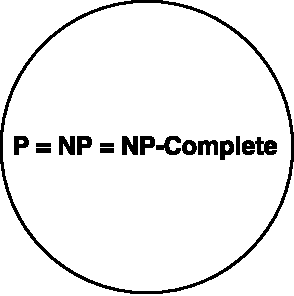
\includegraphics{img/pisnp}

}%
\end{minipage}\hfill{}%
\begin{minipage}[t]{0.45\columnwidth}%
\subfloat[If $P\neq NP$]{\includegraphics{\string"img/Untitled Diagram\string".pdf}}%
\end{minipage}
\caption{Set of complexity classes under different assumptions}
\end{figure}

This conundrum is probably one of the most absorbing problems for
mathematicians. Hundreds of papers were published regarding it, and
none of them came out as proper solution\footnote{For details see: \url{https://www.win.tue.nl/\textasciitilde gwoegi/P-versus-NP.htm}}.
If it could be indeed proven that P is equal to NP, it might be one
of the biggest breakthroughs in modern mathematics. For example most of currently
used cryptography algorithms might become useless.

\section{Boolean Satisfiability Problem}
\label{sec:BSP}

Boolean satisfiability problem, also know as SAT, consists in an attempt to determine
if there exists any substitution of all Boolean variables in a given formula,
so that the whole expression is satisfied. In other words if one can
substitute all variables in Boolean formula so that the result of
expression is TRUE. Usually SAT problem is considered within Boolean
expression built from:
\begin{itemize}
\item Boolean variables,
\item logical operator AND named \textit{conjunction} (usually denoted as $\wedge$),
\item logical operator OR named \textit{disjunction} (denoted as $\vee$),
\item logical negation NOT named \textit{negation} (denoted as $\neg$). 
\end{itemize}
Boolean formula is satisfiable if one can assign Boolean value (TRUE
and FALSE, or 1 and 0 in other words) to every variable in the formula,
so that the whole result stays TRUE.

For simple formulas this problem looks trivial. Consider a formula
\[
x_{1}\vee x_{2}.
\]
It could be easily proven that there
exists at least one possible way to satisfy this formula, for example,
$x_{1}=\mathsf{TRUE}$ and $x_{2}=\mathsf{FALSE}$. The whole formula
is evaluated as $\mathsf{TRUE}$ as a result of this substitution, so it has been
shown that this formula is indeed satisfiable. 

Note that the above formula has in fact \textit{models}, since there exists 3 different interpretations satisfying it. They can be presented with the following truth-table:

\begin{center}
\setlength{\tabcolsep}{6pt}
\begin{tabular}{cc@{\qquad}c}
  $x_{1}$ & $x_{2}$ & $x_{1} \vee x_{2}$ \\
\hline\hline
  $\mathsf{TRUE}$  &   $\mathsf{FALSE}$ &  $\mathsf{TRUE}$ \\
  $\mathsf{FALSE}$ &   $\mathsf{TRUE}$  &  $\mathsf{TRUE}$ \\
  $\mathsf{TRUE}$  &   $\mathsf{TRUE}$  &  $\mathsf{TRUE}$
\end{tabular}
\end{center}
To summarize: a formula -- if satisfiable -- can have more than one model.

On the other hand, consider the  formula:
\[
x_{1}\wedge \neg x_{1}.
\]
It can be easily proven that there  does not exist any interpretation satisfying this formula; it remains $\mathsf{FALSE}$ under any interpretation. Such formulas in logic are called \textit{contradictions}.

Things are getting harder with bigger formulas. In 1971 Stephen Cook
published a paper \cite{Cook:1971}, where SAT, as the  first problem ever,
was proven to be NP-Complete.
Since it is still unchecked if $P=\mathit{NP}$ or not, only exponential-time
algorithms are known \cite{Biere:2009}. If any algorithm was found that
could solve SAT problem in polynomial time, it would mean that all
NP problems could be solved in polynomial time as well \cite{vanLeeuwen:1991}.

\section{The DIMACS format}
\label{sec:dimacs}

In general there are many ways to represent particular instances of SAT problems. Currently,
almost all modern SAT solvers are focusing on specific format of SAT
problems called CNF (Conjunctive Normal Form), as presented in Section~(\ref{sec:CNF}). Let us recall some details of the 
CNF format:
\begin{itemize}
\item Variable -- Boolean variable which can be substituted with one of two
Boolean values, either TRUE or FALSE ($\{x_{1}, x_{2},\ldots, x_{n} \}$)
\item Literal - - a simple Boolean variable with or without a negation (i.e. either $x_{i}$ or $\neg x_{i}$ for $i \in \{x_{1}, x_{2},\ldots, x_{n} \}$)
\item Clause - - disjunction (Boolean OR) of literals (e.g. $x_{1} \vee x_{2} \vee \ldots, x_{k} $)
\item CNF formula -- conjunction (Boolean AND) of clauses; for example
\begin{equation}
\label{equ:ex1}
(x_{1}\vee \neg x_{2})\wedge (x_{2}\vee \neg x_{3}\vee x_{4})\wedge (x_{2}\vee \neg x_{4})\wedge (\neg x_{2}\vee \neg x_{4} \vee x_{5})
\end{equation}
\end{itemize}

Choosing only one format of SAT problems to solve -- the CNF -- is not a restriction, in fact. Recall that all formulas which are not in CNF format can be
transformed into one using simple transformations preserving logical equivalency as described in Section~\ref{sec:CNF}. Of course sometimes
those transformations can explode the formula to huge sizes, but this
is an entirely different problem. 

Having Boolean formula in CNF, it is now necessary to represent it
in a unified, computer-readable format. That is how the DIMACS format was invented \cite{Johnson:1996}.
Within CNF DIMACS format, comments are allowed -- starting with letter
c at the beginning of line. First non-comment line -- called problem
line -- starts with p. Its format should look like this:
\begin{lstlisting}
p FORMAT VARS CLAUSES
\end{lstlisting}
Where:
\begin{itemize}
\item p always must be present (it denotes \textit{problem} line)
\item FORMAT should be CNF (as we consider CNF DIMACS formats). 
\item VARS is number of variables in a given problem
\item CLAUSES is number of clauses present in a given formula.
\end{itemize}

After the problem line, all the following lines are representing clauses.
Each clause is represented with a sequence of integer numbers, where each number describe one variable.
Numbers in each clause are separated with spaces, and can be negated
by adding the \textit{-} character before the corresponding number. Each clause must
finish with 0 at the end.

An example of \textit{CNF DIMACS} format representing the example formula presented above is as follows:

\begin{lstlisting}
c This is comment line
c Another comment line
p cnf 5 4
1 -2          0
   2 -3  4    0
   2    -4    0
  -2    -4  5 0
\end{lstlisting}
The above DIMACS data can be now easily compared with the (\ref{equ:ex1}) formula presented
in tabular form as below:
\begin{equation}
\label{equ:ex1t}
\begin{array}{lc}
(x_{1}\vee \neg x_{2})          & \wedge  \\
(x_{2}\vee \neg x_{3}\vee x_{4}) & \wedge \\
(x_{2}\vee \neg x_{4})          & \wedge \\
(\neg x_{2}\vee \neg x_{4} \vee x_{5})
\end{array}
\end{equation}

\section{Variety of SAT-related problem}
\label{sat-relater}

Currently many problems related to SAT are being solved, some are
just more specific examples of SAT problem, others are more complex
variants.
\begin{itemize}
\item $K$-SAT (where $K$ is a positive integer number), is restricted version of
SAT problem in CNF format, where each clause in the whole formula consists of
no more then $K$ literals \cite{jukna:2013}. It could be generalized to a problem where
each clause consists of exactly $K$ literals, just by adding dummy variables
where the number of literals is less than $K$, and then ensuring that those
variables are FALSE. Some special examples of $K$-SAT are the 1-SAT, which
is trivial and can be solved in linear time just by checking if there
exists at least 2 clauses excluding each other. The 2-SAT problem is also
more trivial then general SAT, being classified as P problem with
polynomial time solutions. The 3-SAT is the first that is already NP-complete.
All other $K$-SAT problems with $K>3$ cannot be easier then 3-SAT nor
can they be harder then the generic SAT problem without any restrictions,
so it can be proven that all $K$-SAT problems with $K\geq3$ are indeed NP-complete.
\item HORN-SAT -- is a specific SAT problem presented in CNF. In horn-satisfiability
each clause in CNF consists of at most one positive literal, and unlimited
number of negative ones. It is proven that the Horn-SAT is P problem with Polynomial,
or even linear time solutions.
\item The 1-in-K-SAT -- this problem is more complex than general SAT problem, as
it tries to determine if there exists assignments to $K$-CNF formula
so that each clause has exactly one true literal. The problem is proven
to be NP-complete.
\item Max-SAT is problem that tries to determinate maximum number of satisfied
clauses with all possible assignments.
\end{itemize}





\section{Current state of SAT-solvers}
\label{sec:stateofSat}

As SAT problem is known to be NP-complete \cite{Cook:1971}, only exponential-time algorithms
are currently known. However, due to the needs of current Information
Technology, new efficient algorithms are being developed. Currently the fastest
SAT-Solvers are capable of solving problems with hundreds thousands
of literals -- thanks to innovative, efficient algorithms. However those achievements
in SAT-solvers are quite new to the world. Not long ago, SAT problems
consisting of 100 clauses would be considered unsolvable. Without proper heuristics,
just by using brute-force algorithm it would give $2^{100}$ combinations
which is approximately $2*10^{30}$. Not even modern
super-computers would be capable of solving that in reasonable
time.

SAT solvers are being developed in many institutions simultaneously.
There was demand to create a way to compare those solvers. Due to
this need each year a competition  called SAT competition is held \cite{Satcomp}.
On this event, each signed up solver is challenged on chosen track
by numerous benchmarks to emerge the fastest one. Last competition
was held in 2017 and the main track was won by Maple Solver\footnote{\url{https://sites.google.com/a/gsd.uwaterloo.ca/maplesat/maplesat}}. Some other worth mentioning popular solvers include:
\begin{itemize}
\item Minisat \footnote{\url{http://minisat.se/}},
\item Glucose \footnote{\url{http://www.labri.fr/perso/lsimon/glucose/}},
\item Riss \footnote{\url{http://tools.computational-logic.org/content/riss.php}},
\item Lingeling \footnote{\url{http://fmv.jku.at/lingeling/}},
\end{itemize}
but there are many other interesting implementations as well.



\chapter{Basic SAT Processing}
\label{chap:Heuristics}

\section{Preprocessing}
\label{sec:Preprocessing}

When SAT Solver is being run, the very first thing that has to be
done is input reading. Program needs to read DIMACS\footnote{See \ref{sec:dimacs} for more information} file, parse all
clauses and it might or might not check for inconsistencies. For example,
if clause number (or variable number) matches with those given in
problem line. It is however debatable if this steps can be considered
a part of the whole algorithm, as there is not much to optimize. Also
providing correct input is the user's responsibility and solvers do not
have to provide any assurance that those inconsistencies will be detected
or that result will be correct. 

After parsing  the input data, the next step for SAT solver might be called
\textit{preprocessing}. The main  purpose of that step is to scan all data that
was given as an input and find out if there might be any simplifications
that can be done in linear or polynomial time. There are of course many possible ways to do it,
and the one explained below might be considered as one of the simplest.
Those algorithms can constitute  also a part of more complex algorithms in execution
phase.

\subsection{Unit Propagation}
\label{subsec:UnitProp}

One of the easier ways to simplify the problem is to find possible
substitutions in linear time. For example, it can be a  pre-scan in search of unit-clauses.
Unit-clause is a clause that consists of exactly one literal \cite{Franco:1993} -- so one
variable or negated variable. Considering DIMACS example:

\begin{lstlisting}
p cnf 3 4
 1 -2    0
 1  2 -3 0
       3 0
-1    -3 0
\end{lstlisting}

There are 4 clauses: 
\begin{gather}
x_1 \vee \neg x_2, \\
x_1\vee x_2\vee \neg x_3, \\
x_3\label{equ:clause3}, \\
\neg x_1 \vee \neg x_3
\end{gather}
If there exists Satisfiable model of this formula -- all clauses have to resolve as $\mathsf{TRUE}$.
Considering the 3-rd clause (\ref{equ:clause3}), it contains exactly one literal: $x_3$. The solver has
to substitute the $\mathsf{TRUE}$ value for the  $x_3$ variable, so that the 3-rd clause
is satisfied. Subsequent substitutions should be carried out  for any occurrence of this variable in a consistent way and the clause should be simplified. In the considered example this results with:
\begin{gather}
x_1 \vee \neg x_2, \\
x_1\vee x_2, \\
\label{equ:clause3reduced}, \\
\neg x_1 
\end{gather}
Therefore our search space has been  reduced by 1 variable
already (and one clause); some clauses have been shortened. This procedure can be repeated as long as there is still at least 1 unit clause in formula.

\subsection{Pure Literals}
\label{subsec:Pure}

There is another example of a possible way to simplify a given input formula. The whole reasoning
behind it is to find out if there exists a variable, that occurs exclusively
as positive variable, or exclusively as negative variable \cite{Biere:2009}. Consider the
following example:

\begin{lstlisting}
p cnf 3 4
 1  2    0
 1  2 -3 0
    2  3 0
-1    -3 0
\end{lstlisting}

All the solver has to do is to keep track of each variable. In this
example, variable number 2 occurs within 3 clauses: the 1st, the 2nd and the 3rd.
In each of these clauses it occurs as a positive literal (without negation).
Knowing that, by assumption that solver is looking for satisfying
substitution, $\mathsf{TRUE}$ value can be assigned to $x_2$. It is possible
only because the idea behind solvers is to find at least one satisfying
solution. If the solver had to find all possible solutions pure literals rule
cannot not be used, as the solver might miss a solution where $x_2$
is $\mathsf{FALSE}$.

\subsection{Clause Resolution}
\label{subsec:Clause-evaluation}

Transformations of clauses are very wide and difficult topic to discuss.
As with all
algorithms like that, the biggest challenge is to balance the usefulness
with time consumption. Also, transforming clauses by any means may be quite
dangerous for the whole algorithm, as it is easy to change satisfiability
of the original formula \cite{Biere:2009}.

The main issue, as mentioned above -- is usefulness. It is under debate
what clauses are the most useful for the solvers. The solver could redefine
almost every clause in the original problem, but the question remains
-- will it be more useful then the previous state? The safest approach
to this problem is just to remove obsolete information that certainly
does not help in any way. Solvers can easily remove obsolete clauses.
Consider the following two clauses:
\begin{equation}
(x_1 \vee x_2)\wedge(x_1\vee x_2\vee x_3)
\end{equation}
It is clear that the second clause is similar to the first one, but with some
overhead. If the whole formula needs to be true -- then $(x_1 \vee x_2)$ has to evaluate to true as well. It means that an overhead $x_3$ in second clause brings no new information,
thus the whole clause can be safely removed from the formula\footnote{This relation is called Subsumption, or Syllogism. See \url{https://en.wikipedia.org/wiki/Syllogism} for more references.}
\begin{equation}
(x_1 \vee x_2)\wedge(x_1\vee x_2\vee x_3)\equiv x_1 \vee x_2
\end{equation}
Another way of removing obsolete information is to find clauses that
cancel themselves out. Considering given clauses:
\begin{equation}
(x_1 \vee \neg x_2)\wedge(x_1\vee x_2)
\end{equation}
The truth table for the above example is as follows:
\begin{center}
\setlength{\tabcolsep}{6pt}
\begin{tabular}{ccc}
  $x_{1}$ & $x_{2}$ & $(x_1 \vee \neg x_2)\wedge(x_1\vee x_2)$ \\
\hline\hline
  $\mathsf{TRUE}$   &   $\mathsf{TRUE}$  &  $\mathsf{TRUE}$  \\
  $\mathsf{TRUE}$   &   $\mathsf{FALSE}$ &  $\mathsf{TRUE}$  \\
  $\mathsf{FALSE}$  &   $\mathsf{TRUE}$  &  $\mathsf{FALSE}$ \\
  $\mathsf{FALSE}$  &   $\mathsf{FALSE}$ &  $\mathsf{FALSE}$
\end{tabular}
\end{center}
With a quick look in the truth table, it is visible that
the final solution is equal to $x_1$ value, and $x_2$ does not really matter.
Thus this clauses can be reduced to one clause
without losing any information, as they are logically equivalent (\ref{sec:implication})
\begin{equation}
(x_1 \vee \neg x_2)\wedge(x_1\vee x_2) \equiv x_1
\end{equation}
This can of course be proven by basic Boolean transformations as well.

There are also some possibilities to gather new information. There
is a simple way of generating new clauses without changing satisfiability state,
or losing any information. Consider clauses:
\begin{equation}
(x_1 \vee \neg x_2)\wedge(x_2\vee x_3)
\end{equation}
And now substituting $x_2$ (and keeping satisfiability of that formula):\\
$x_2=\mathsf{TRUE} \Rightarrow x_1= \mathsf{TRUE}$ ($x_3$ did not matter)\\
$x_2=\mathsf{FALSE} \Rightarrow x_3= \mathsf{TRUE}$ ($x_1$ did not matter)\\
It is clear that either $x_1= \mathsf{TRUE}$ or $x_3= \mathsf{TRUE}$.
Transforming that into one clause we have $x_1\vee x_3$.
It can be safely added to the whole formula, and
satisfiability status is not alternated\footnote{This example is again just showing a use of propositional resolution, described in section \ref{sec:resolution}}.
\begin{equation}
(x_1 \vee \neg x_2)\wedge(x_2\vee x_3)\equiv (x_1 \vee \neg x_2)\wedge(x_2\vee x_3)\wedge(x_1\vee x_3)
\end{equation}
Those transformations are usually expanding our problem - giving
new clauses that might or might not help in the future. This way of
adding new information is controversial as it is hard at this point
to tell if the new clause will be anyhow useful. Hence, taking into account that searching
for those kind of clauses might be time consuming, it is not always
worth to do so.

\subsection{Sub-problem breaking}
\label{subsec:subbreaking}

Breaking SAT problem into smaller problems is very complicated and
comprehensive topic. Considering example:
\begin{equation}
(x_1 \vee x_2)\wedge(x_3\vee x_4)
\end{equation}
the size of the entire search space is equal to $2^4=16$. However
in this example there are no connections between the 1st and the 2nd clause.
These clauses are disjunctive, so they can be considered separately.
To better describe this problem, consider the given below example:
\begin{equation}
(x_1 \vee x_2)\wedge(\neg x_1\vee x_2)\wedge(x_3 \vee \neg x_4)\wedge(x_3\vee x_4)
\end{equation}
Here again, the size of the search space is equal to 16. However like in the former example above
-- it is possible to distinguish 2 separate sub-problems. The first sub-problem
$(x_1 \vee x_2)\wedge(\neg x_1\vee x_2)$
and the 2nd sub-problem $(x_3 \vee \neg x_4)\wedge(x_3\vee x_4)$ are independent.
It is so due to the lack of variables that can be found in both
of those sub-problems. Now, having 2 separate sub-problems - the necessary
condition for the whole formula to be satisfiable is that each of sub-problems
is satisfiable on its own. 

However finding if sub-problem is satisfiable
is noticeably easier -- in the example above, decreasing one problem with
search space with $2^4$ to two problems with search
space $2^2$. Considering general example, having n
variables, the size of the search space is equal to $2^{n}$. Distinguishing
separate problem with m variables, the search space is decreased, leaving
2 problems with combined search space $2^{n-m}+ 2^{m}$ which
can be much smaller by  considering large enough $m$.

The above example seems very promising, however the biggest downside of it
is that it takes a very optimistic assumption -- that it is possible
to find two completely separate sub-problems, which is very unlikely.

There is a way though, to break bigger problems into smaller sub-problems
in  more generic way. If we can find as few variables as possible
that are responsible for connectivity of the set of all clauses,
there would be a way to create iteration of sub-problems. Such algorithms
are called cut-set techniques \cite{cut-set}. Their purpose is to find the minimal number of 
cuts in the graph, to break it into 2 separate graphs.

Having $2^{m}$ possible
solutions: if there exists a variable that could be assigned to break
the whole problem in two parts, the initial formula can be reduced considerably
as shown on the graph presented on the next page.

Considering $n+1$ variables, if 2 equally big problems can be designated
after removing 1 variable, the search space is reduced from $2^{N+1}$ to
$2^{(N/2) + 2}$. All that needs to be done is to assign
2 possible values to that one variable -- $\mathsf{TRUE}$ and $\mathsf{FALSE}$. After the assignment,
the problem is analogous to the previous example with 2 separate sub-problems.
All that needs to be checked is if after the assignment to this one variable,
any of newly created problems is satisfiable. If yes, the entire problem
is satisfiable by the values calculated as a solution to sub-problem
and the one variable with value assigned to it. Of course it is very
difficult to find a correct pivot variable (or a set of such variables) that
could create completely separate sub-problems after the assignment. The
best possible way to do so is to create a graph of dependencies of variables.

Consider the  following example:

\begin{lstlisting}
p cnf 7 8
 1  2  3             0
-1 -2 -3             0
 1    -3 -4          0
          4  5  6    0
          4 -5       0
                6  7 0
            -5  6    0
             5    -7 0
\end{lstlisting}
graph of variables' dependencies can be created, with variables as
nodes and clauses as paths:

\begin{figure}[H]
\begin{centering}
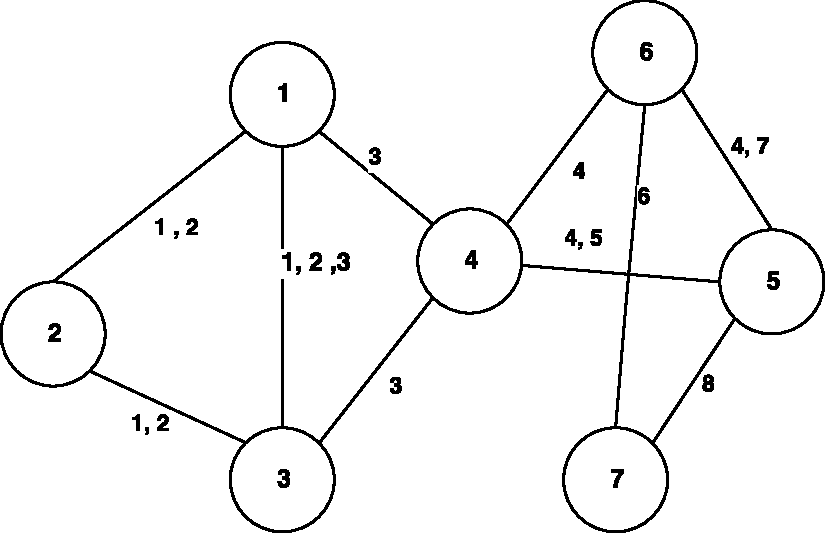
\includegraphics{img/graph1}
\par\end{centering}
\caption{Graph of dependencies}
\end{figure}

It is visible that variable with number 4 can break this graph into
2 separate parts alone. Given that the problem consists of 7 variables, it makes us to examine 128 possible solutions. If variable 4 is assigned, either
$\mathsf{TRUE}$ or $\mathsf{FALSE}$, it creates 2 sub problems, with 8 possibilities each, and so only 16 possible solutions to check. 

\begin{figure}[H]
\begin{centering}
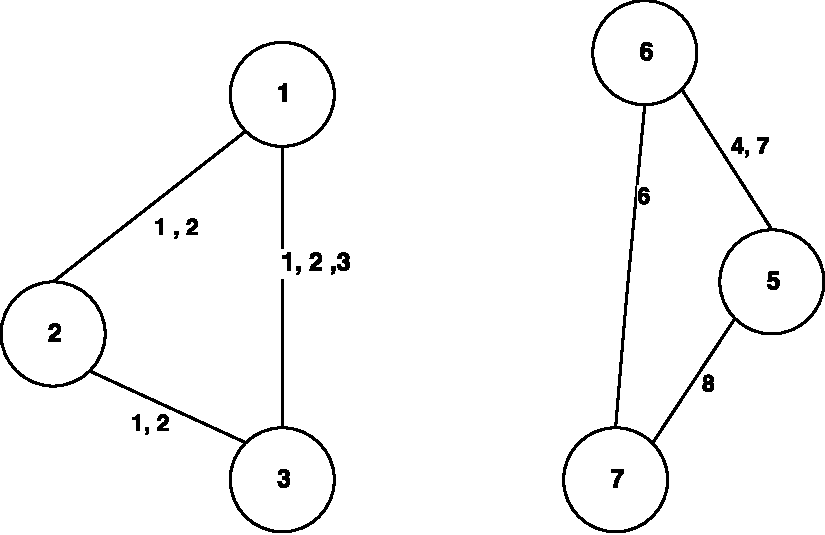
\includegraphics{img/graph2}
\par\end{centering}
\caption{Graph of dependencies after the first assignment}
\end{figure}
However, as it is unknown what substitution could give SAT solution,
so both TRUE and FALSE have  to be considered as a possible assignments to variable 4; this leads
to 32 possible solutions to check, comparing to $2^{7}=128$ in the original problem.

The main issue here is exactly the same as with the previous heuristics. The
biggest downside is to get to know if it is worth to even look for
such pivoting variables. Finding paths that are essential for consistency
of graph is hard and time consuming -- especially considering the size
of average SAT problems with thousands of variables and hundreds of
thousands of clauses. There is also possibility that no such variable
even exists, and the whole process remains pointless. Taking that
under consideration, this technique might be considered useful only
in very specific types of crafted problems.

\section{Execution part}
\label{sec:Execution}

With all trivial variables removed,the  next step is to look for a solution
for all the remaining variables. This is the main part of program which takes
majority of time for  execute.

\subsection{Brute Force}
\label{subsec:Brute}

Brute force search is of course the easiest and most straightforward way to look for an admissible
substitution. If the solver checks all possible substitutions and finds
that none of those evaluates formula as true, then the formula is unsatisfiable.
Otherwise it returns the  first  satisfying substitution found during the search procedure. This is
of course very naive approach, because as stated before -- with even
100 variables there are $10^{30}$ possibilities to check, 
which is  too much for any computer to evaluate.

But as SAT is proven to be NP~\cite{Cook:1971}, so in theory every existing algorithm has
exponential time of execution. So why brute forcing is not working? The main difference with respect to more efficient approaches consists in application of efficient reduction techniques.
 Sophisticated heuristics are able to significantly reduce the size of the search
tree, while brute force search will just look at every leaf which is drastically inefficient.

\subsection{The DPLL Algorithm}
\label{subsec:DPLL}

The Davis–Putnam–Logemann–Loveland Algorithm \cite{Biere:2009} is an enhancement of previously
developed DP algorithm. Its main properties are that it is based
on searching binary tree with chronological backtracking. Comparing
it to brute force search, it allows to skip huge parts of search
space. Of course as the whole SAT problem is NP, the DPLL algorithm -- as every
NP-complete algorithm -- has exponential time in the worst case
scenario. However in most cases it works much faster and it was huge
breakthrough in SAT solvers world. Also DPLL is generally based on
heuristics presented before, unit clause propagation\footnote{Head to \ref{subsec:Clause-evaluation} for more information} and Pure
Literals evaluation.\footnote{Head to \ref{subsec:Pure} for more information}

If there exists at least one Unit Clause, it might
be satisfied by assigning correct value. The same thing goes with Pure
Literal - those can be assigned to satisfy all clauses that contain
this literal. So with each decision, the algorithm will choose those variables
that can get assignment with correct value. To show some example,
consider the following clauses presented in DIMACS format:

\begin{lstlisting}
 1  2       0
-1 -2 -3  4 0
 1    -3 -4 0
 1     3 -4 0
   -2  3    0
   -2 -3    0
\end{lstlisting}
And its algebraic representation:
\begin{equation}
\label{equ:algver1}
\begin{array}{lc}
(x_{1}\vee x_{2})          & \wedge  \\
(\neg x_1\vee \neg x_{2}\vee \neg x_{3}\vee x_{4}) & \wedge \\
(x_{1}\vee \neg x_{3}\vee \neg x_4)          & \wedge \\
(x_{1}\vee x_{3}\vee \neg x_4)          & \wedge \\
(\neg x_{2}\vee x_{3})          & \wedge \\
(\neg x_{2}\vee \neg x_{3})
\end{array}
\end{equation}
And to break down how it is proceeded by the DPLL algorithm, consider that the  solver
picks a variable and value. As there are no Unit Clauses nor Pure
Literals the first variable and value are picked arbitrarily. In this example
$x_1$ is taken, and the value $\mathsf{FALSE}$ is assigned to it.
The formula changes as follows, with satisfied clauses removed: \footnote{Only DIMACS format
will be presented from now on, as it is more readable}

\begin{lstlisting}
 2       0
   -3 -4 0
    3 -4 0
-2  3    0
-2 -3    0
\end{lstlisting}
Now, observe that the  first clause is a Unit Clause - to satisfy it, $x_2$
has to be assigned $\mathsf{TRUE}$ which results in:

\begin{lstlisting}
-3 -4 0
 3 -4 0
 3    0
-3    0
\end{lstlisting}
It is obvious that with those previous substitutions, the 3rd and the 4th
clause cannot be satisfied at the same time -- as variable $x_3$ cannot
be simultaneously $\mathsf{TRUE}$ and $\mathsf{FALSE}$. It is time to backtrack to the
previous variable that was chosen arbitrarily, i.e. the $x_1$
(as the remaining variables were chosen due to pure literals or unit
clauses) and assign of the  $\mathsf{TRUE}$ value to it (as previously false was assigned). The new result is:

\begin{lstlisting}
-2 -3 4 0
-2  3   0
-2 -3   0
\end{lstlisting}
Here with this substitution, both $x_2$ and $x_4$ are satisfying the definition of Pure Literals
and can be assigned $\mathsf{FALSE}$ and $\mathsf{TRUE}$ respectively leaving empty formula.
It means that this formula is satisfied by:
\begin{center}
\setlength{\tabcolsep}{6pt}
\begin{tabular}{c|c|c|c}
  $x_1$   &   $x_2$ & $x_3$   &   $x_4$   \\
  \hline
  $\mathsf{TRUE}$  &   $\mathsf{FALSE}$ & $\mathsf{TRUE}\vee \mathsf{FALSE}$\footnotemark  &   $\mathsf{TRUE}$ 
\end{tabular}
\footnotetext{\label{foot:tab}$x_3$ was not assigned during the whole process. It means that its value does not matter within the rest variables assigned that way}
% the whole footnotes here are kind of confusing for me. I can not make anything else to work, and this solution is far from perfect
\end{center}
To illustrate how the actual search space was reduced, a binary
tree can be used:
% here the label did not work for me when it was inside figure. No idea why.
\label{fig:DPLL}
\begin{figure}[H]
\begin{centering}
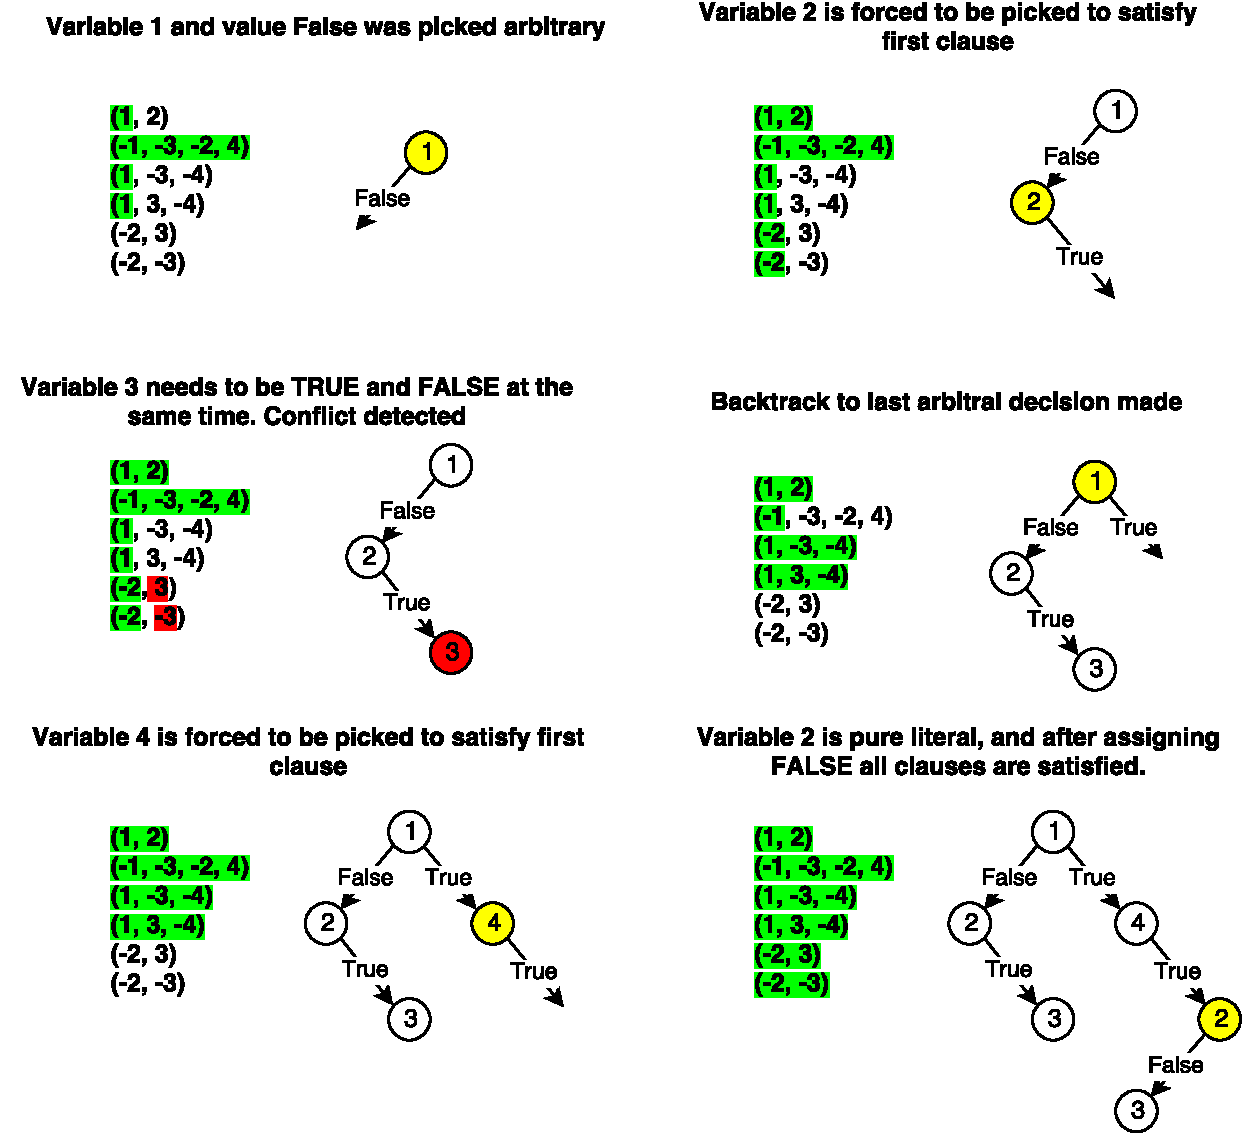
\includegraphics[scale=0.75]{img/dpll_graph}
\par\end{centering}
\caption{DPLL -- graph of decisions}
\end{figure}


\subsection{The CDCL Algorithm}
\label{subsec:CDCL}

The CDCL (Conflict Driven Clause Learning)\cite{Biere:2009} Algorithm was a new, modern
and more faster approach to SAT solving. It was a huge step forward
in terms of finding solution of a SAT problem. The main idea of CDCL
was to improve heuristics brought in by DPLL, improve them and allow
the solver to evolve, based on the input formulas. The idea started when it
was discovered, that in the DPLL algorithm, solvers were wasting a lot
of time doing the same comparisons and the same operations on different branches
of a tree, which was very inefficient. To improve its performance,
the CDCL algorithm was developed. It was able to learn basing on conflicts
it found. The algorithm bases on some 4 basic heuristics:
\begin{itemize}
\item Variable choosing;
\item Value choosing;
\item Non-chronological backtracking;
\item Restarts.
\end{itemize}

\subsubsection{Variable choosing}
\label{subsubsec:Variable}
The first issue in CDCL algorithm is very similar to the one present
in DPLL. The main question is about the order in which the  variables are selected
for substitution. In other words, the question is which order is the best for a given formula and
how to find the optimal sequence (order). Thanks to the new properties of CDCL, this
problem becomes less important then it was before. In DPLL, if the
first variable was chosen incorrectly, the whole sub-tree  of a tree (located below the choice point) had
to be searched to get back to the starting point. However in CDCL it is
sometimes even desirable to choose incorrect variables in specific
order so that conflicts are found as fast as possible. Some of the
basic ideas to choose variables could be:
\begin{itemize}
\item Random, or in order -- Randomly pick any value, or always take the first one;
\item Based on number of appearances -- Pick the variable that appears in the most clauses;
\item Based on differences between signing -- Pick the variable that the difference of occurrence as positive and negative literal is the biggest;
\item Based on reduction -- Pick the variable that will reduce the most clauses in formula.
\end{itemize}

\subsubsection{Value choosing}
\label{subsubsec:Value}
This problem is correlated with the previous one. If the solver chooses
a variable to be assigned, then the next decision is to choose which
value should be assigned to it first -- of course if there is
such possibility. With unit clause or pure literal strategy, the value as well
as the variable is imposed. Also if chosen variable was assigned in a given 
combination, its value is imposed as well. 

As the value can be either $\mathsf{TRUE}$ or $\mathsf{FALSE}$, usually the solver can bring
on 2 strategies -- excluding trivial ones, like assigning always  $\mathsf{TRUE}$
or always $\mathsf{FALSE}$. The first strategy is more obvious one -- the solver looks
for the actual solution. Considering variable that appears -- e.g. 9 times
in 9 different clauses, in 8 as positive literal and in 1 as negative.
Intuitively, assigning the  $\mathsf{TRUE}$  should be a better solution. It would satisfy
8 of the given clauses, which in theory, should bring the solver closer to the solution. 

By doing so however, the solver removes some valuable information. It might
end up being stuck in some part of a tree, and it might have to search
it to the very end to find that the intuitive substitution was a wrong one. 
 With the very same example -- with 9 appearances of variable,
1 as negative literal and 8 as positive, the solver could also assign
$\mathsf{FALSE}$ to it. It allows to reach potential conflict much faster and
the solver can learn new clauses and save precious time in next branches.

\subsubsection{Backtracking}
\label{subsubsec:Backtrack}
This is where CDCL solvers starts to distinguish itself from DPLL
solvers. In DPLL backtracking was simple -- based on the Depth-First Search (DFS) graph-searching algorithm.
If solution was not found, or conflict was detected, the algorithm
backtracks as long as there are possible assignments. This kind of
backtracking is also known as \textit{chronological backtracking}.

CDCL solvers are also using backtracking when conflict is detected, but it is a not chronological backtracking.
It does not fall back to the first possible node -- but to the node that fits 
certain restrictions. Basic algorithm is constructed
in such a way, that newly learned clause is used as soon as possible.

\subsubsection{Restarts}
\label{subsubsec:Restart}
Restarts are crucial part of the CDCL solver. It was discovered, that
solvers were loosing most of its time by looking at the wrong branches
in search tree. If there are 100 variables, and the solver chooses the
wrong value for the very first variable, then it would basically had
to search $2^{99}$ combinations to find out the mistake. 

To save solvers from such problematic dead-end searching, it was discovered
that the solver could restart itself -- this means  that it would start building
search tree from the very beginning, saving its learned clauses and
other gathered information. This allows the solver to get out of dead-end branches,
by recreating the entire tree, yet, when restarts are introduced,
there are still some questions to answer. The most important are to
know when exactly the solver should restart itself. There are still some
disputes about algorithms defining it. Usually restarts depend on
a number of clause learned. Some modern SAT solvers also introduced
random restarting to prevent long tailing. 

With restarts, however, new problems appeared. If clause learning
process is behaving incorrectly, so that no new information was gathered
with each conflict, restarts can easily end up in an infinite loop. The second
problem is to determine whether a given formula is indeed UNSAT. Without
restarts, all the solver had to do was to search the whole search-space
of the problem. With restarts introduced, the solver will most likely
restart itself without reaching the end of a tree. 

\subsection{Modern CDCL Algorithms}
\label{subsec:ModernCDCL}
In previous chapters all heuristics introduced are the core of CDCL
solvers. However, based on many years of research and numerous experiments,
some new heuristics were introduced~\cite{Biere:2009}. Most of them are just enhancements
of the presented ones, but they do make modern solvers unbelievably efficient.
Some of them will be described briefly below:
\begin{itemize}
\item Lazy data structures -- Data structures that are updated as they are actually needed \cite{alsinet2004max};
\item Clause deletion -- Reducing the clause that are learned to the absolute minimum \cite{sorensson2009minimizing};
\item Branching heuristics -- optimizing branching within a tree for a clause learning purposes \cite{liang2016learning};
\item Look-ahead heuristics -- With each variable, both $\mathsf{TRUE}$ and $\mathsf{FALSE}$ values are assigned and results are compared \cite{heule2011cube}.
\end{itemize}

\chapter{SAT Solver Implementation}
\label{chap:Impl-4}

\section{General Notes and Program Structure}
\label{sec:ProgramStructure}

The programming language chosen for implementation of the experimental
SAT-Solver is Python 3. Throughout the whole implementation and testing process,
Python version 3.6.1 was used and it is not guaranteed that it
will work with any other version. Specifically Python 2 interpreters
will not work, due to lack of backward compatibility between Python
in version 3 and version 2\footnote{See \url{docs.python.org/release/3.0.1/whatsnew/3.0.html} for some basic comparisons}. All Packages used were internally implemented,
or are available in Python Standard Package Library -- which means
that no external packages need to be downloaded to launch code.

Here is a list of the Standard Package Libraries that were used:
\begin{itemize}
\item Math library\footnote{\url{docs.python.org/3/library/math.html}} for copysign function and \textit{INF} constants;
\item Copy library\footnote{\url{docs.python.org/3/library/copy.html}} for deepcopy function;
\item Heapq\footnote{\url{docs.python.org/3/library/heapq.html}} for Heap queue algorithm;
\item Enum\footnote{\url{docs.python.org/3/library/Enum.html}} for Enumeration type;
\item Os\footnote{\url{docs.python.org/3/library/os.html}} and sys\footnote{\url{docs.python.org/3/library/sys.html}} libraries for system depended calls;
\item Argparse\footnote{\url{docs.python.org/3/library/argparse.html}} for parsing command line arguments.
\end{itemize}
Also for testing purposes libraries \textit{sub-process}\footnote{\url{docs.python.org/3/library/subprocess.html}} and \textit{time}\footnote{\url{docs.python.org/3/library/time.html}} were used
to call solver as external process and measure time spent on execution.

In general, the whole project contains 4 major code files.
\begin{itemize}
\item aghSolver.py is the main executable file. It contains all details of user interface as well as input validation; 
\item tree.py is the file that contains all functions responsible for algorithmics; 
\item node.py is a helper file containing support classes and functions that did not interfere with the main data structure;
\item functionRegister.py is responsible for gathering information about replaceable functions within algorithms.
\end{itemize}
More details of implementation will be presented in the following sections.

\section{Data Structures and initialization}
\label{sec:DataStrcuture}

In this chapter data representation issues will be presented. Note, that data
structure called \textit{list} in this chapter does not mean commonly
known linked list data structure, but build-in Python type called
list. With respect to implementation Python list  is more similar to vector
data structure -- with O(1) access time complexity and O(1) amortized
appending time complexity\footnote{https://www.ics.uci.edu/~pattis/ICS-33/lectures/complexitypython.txt}.

For optimization purposes CNF clauses will be represented in 2 different
ways, and those representations have to stay consistent throughout the
entire execution. The first representation know as \textit{Clauses} or \textit{Current
Clauses} is a simple mapping of CNF clauses into list of lists. This
variable is list of all clauses, where each clause is a list of all
literals -- negated if necessary. So the length of list is always constant
and equal to the number of clauses (not necessarily number of clauses
encoded in DIMACS file). It will be expanded with each learnt clause.
If any clause is satisfied during execution, it is noted as empty list.


The second representation, which was mentioned
before, has to be consistent with the first one, is a look-up-oriented representation.
It is a list of all variables in the SAT Problem, where each variable is
represented as a list of clauses in which this clause can be found.
Here also each number can be negative if the literal within a clause is
negative. This list always remains with the same size -- no new variables appear during the execution.
If variable is removed from the formula (Substituted by any value), its look-up entry will
become an empty list.
To show exactly how those structures are constructed, consider
the following CNF example\label{misc:datastructexample}:

\begin{lstlisting}
p cnf 3 5 
 1  2  3 0 
-1 -2 -3 0
-1    -3 0 
-1     3 0 
 1    -3 0
\end{lstlisting}
In the example above, the data structures look like this:
\begin{itemize}
\item clauses: {[}{[}1, 2, 3{]}, {[}-1, -2, -3{]}, {[}-1, -3{]}, {[}-1,
3{]}, {[}1, -3{]}{]}
\item variable\_lookup: {[}{[}1, -2, -3, -4, 5{]}, {[}1, -2{]}, {[}1, -2,
-3, 4, -5{]}{]}
\end{itemize}
As mentioned before, those structures are actually representing exactly the
same  data, so with each update of one of those representations, the second one has
to be updated as well.

The main data structure used for  solution searching is a binary tree.
The  structure under each node consists of at most 2 children. It is a very simple,  intuitive
structure to use for searching a solution for SAT problem as each
variable can have one of two Boolean states. 

To represent each node
in the Tree -- Node class was implemented. The class does not contain any
logic, only raw data is used. To construct a Node, a variable instance (described
below in this chapter) is needed. Also if the Node is not a root of
a tree -- reference to its parent node can be passed as optional argument.

Information held within Node are:
\begin{itemize}
\item variable -- instance of Variable class strictly connected with this
node,
\item parent -- reference to parent node (\textit{None} if root of tree),
\item variable\_lookup\_valid\_for\_node and current\_clauses -- clause representation
valid for node,
\item left\_checked and right\_checked -- Indicators if search in given part
of a tree was completed\footnote{It is important that those variables
should be set to true value only when solver is sure that nothing
is left to be searching within corresponding branch},
\item left\_child and right\_child -- references to children of the 
node\footnote{Important note: left\_child is corresponding to a path in which TRUE
value was assigned to current node, and right\_child means FALSE value
was assigned}, 
\item tree\_depth -- value indicating depth of the tree in which node is
located.
\end{itemize}
The Node class holds also all of its own instances within static variable.
This is necessary to optimize memory usage while restarting the solver.
This allows to quickly remove all nodes when they are no longer needed.

Second helper class is Variable, which, as mentioned before, is strictly
connected with Node variable. From programming point of view they
could even  be joined together to a single class, however, due to logical
separation, they where distinguished. Also, a major advantage of this
class is that all Variable class instances are created at the beginning
of the program. This way it can hold all information available from the
very beginning (like initial occurrences and number of variables that
each instance is corresponding to), whereas Node instances are created
and destroyed dynamically.

The main functionalities bounded with tree data structure are located
within Tree class, in tree.py file. This class is responsible for
managing all functions that have any impact or that take any information
from the main binary tree object. The most notable members of this class
are Tree pivots: main\_node and current\_node which are references
to top level of the tree and currently considered, \textit{pivot}, node. Also, all clauses
and variables within problem -- (also in lookup form which was explained
before, \ref{misc:datastructexample}), and many variables that are needed for iterative searching
process throughout binary tree.

\section{API}
\label{sec:API}

As mentioned before, many functions within the search tree are replaceable.
This section will explain how  this mechanism is implemented, how to
implement functions that could replace the existing ones, and how to create
a new family of functions.

\subsection{API implementation}
\label{subsec:APIimpl}
The goal of implementing a common interface for functions is to minimize
changes that need to be done after a new function is created. With
the current solution, all that needs to be done is to create a function
that uses interface as shown below, and use python decorator\footnote{See \url{https://wiki.python.org/moin/PythonDecorators} for documentation of decorators} to register
this function as a replacement function. First thing to note is that
within functionRegister file there is Enumeration object that translates
the type of a given function into integers. 

\begin{lstlisting}
class FunType(Enum):     
	VALUE = 1
	VARIABLE = 2
	BACKTRACK = 3
	RESTART = 4
\end{lstlisting}
So, as shown above, there are currently 4 types of functions that can
be replaced:
\begin{itemize}
\item Value functions -- functions responsible for picking the next value to
be used by the solver (used after the Variable was picked),
\item Variable functions -- functions responsible for picking the next variable
to be used by solver,
\item Backtrack functions -- most complex set of functions which are responsible
for backtracking whenever a conflict was detected,
\item Restart functions -- functions that determine conditions at which the solver should
restart itself.
\end{itemize}
With those function types, each replaceable function can be decorated
with the following set of  parameters:
\begin{lstlisting}
@register(type, cli_argument, help_description)
\end{lstlisting}
where:
\begin{itemize}
\item type -- is a value from enum presented on previous page, encoding the type of the function,
\item cli\_argument -- is a string that will be used by the user to choose this
function within its function group,
\item help\_desc --- is a help string
that user will see after using long help option.
\end{itemize}
As an example consider the following specification:
\begin{lstlisting}
@register(FunType.VALUE, cli_arg='F', help_desc="Return always FALSE value") 
def return_false(self):         
	return False
\end{lstlisting}
This function is marked as a VALUE function so its responsibility is
to pick a value that will be used by the solver. Its command line
argument is F, so it will be used when the user launches the solver with argument
–Value=F. Help\_desc will be presented to the user after using -l or –long\_help
option.

This decorator handles a lot of functionality, which enables a
quick implementation of new functionalities. Everything that needs
to be done after adding new functions is handled by it. Using this
construct automatically allows the user to chose it within given function
family, as well as places the help description string in \textit{long-help}\footnote{calling solver with -l or -long\_help option} in the right place.
However, each family function has its own restrictions that will be
pointed out later on  in this chapter.

A more difficult task is to implement a new family of functions. Here is a list of things that have to be done:
\begin{itemize}
\item Extend Enum within function\_register file. 
\item The wrapper function in aghSolver file needs to be extended
with a new \textit{elif} and a new list of functions inside that file needs to
be created.
\item New argument needs to be added within the parser() function with proper choices
which should be taken from the function list created before.
\item The new function needs to be accepted by the Tree object class constructor,
which enforces passing it within the run\_solver function. 
\item The function is available within the Tree Class constructor and can
be assigned to some default function by its name. \footnote{Important note
is that default value of parameters are handled within parser() function,
not within Tree class constructor.}
\end{itemize}

\subsection{API functions limitations and requirements}
\label{subsec:APIfuncts}
In this part all replaceable functions families will be described.
Each of them has its own requirements regarding functionalities which
they can perform on the  main tree structures as well as return values.
All those requirements need to be followed to ensure integrity of the 
Tree structure. The following table is added to sum up all the implemented function
families. The detailed argumentation and description is available in corresponding
sub-chapters.

\begin{table}[H]
\begin{centering}
\begin{tabular}{|c|c|c|}
\hline 
Function Family & Return value & Logically constant\tabularnewline
\hline 
\hline 
Variable & Variable object, or None & Yes\tabularnewline
\hline 
Value & True or False & Yes\tabularnewline
\hline 
Restart & True or False & Yes\tabularnewline
\hline 
Backtrack & nothing & No\tabularnewline
\hline 
\end{tabular}
\par\end{centering}
\caption{Replaceable function description}

\end{table}


\subsubsection{Variable functions}
\label{subsubsec:Varfuncs}
All variable functions are required to return a valid Variable instance
for the  current state of a tree. The simplest way to achieve this is by
gathering variables from variables\_to\_use member of the Tree class.
It ensures that the variable to be returned is valid and still usable. However
those functions are not supposed to modify anything within the Tree class;
in particular, they are not responsible for removing object from variable\_to\_use
list. Each of those functions could be marked as constant if the solver
was implemented in C++. An important note is that if there is no valid
Variable to be returned (which means variables\_to\_use list is empty),
the None object has to be returned.

\subsubsection{Value functions}
\label{subsubsec:Valfuncs}

Those functions, similarly to Variable functions are not supposed
to edit any of the members within Tree Class. Their return value should be
either True or False, depending of which value was chosen. Important
note is not to return any other objects then Boolean, in particular
None objects Empty lists or integers even though they could be treated
as Boolean value within Python language. Main source of information for this
functions is variable that was chosen and it can be accessed using
latest\_var member of a Tree class.

\subsubsection{Restart functions}
\label{subsubsec:restartfuncs}

Restart functions are responsible for detecting if a  restart of the  Solver
should be performed or not. Their return value is either True, if
restart should be performed in next iteration or False if restart
should not be performed. Check out Restart section within 3.2.3 for
more details of restarts within CDCL SAT solvers.

\subsubsection{Backtrack functions}
\label{subsubsec:Backfuncs}

Those are most complicated functions of all. Also those are the only
functions that have big impact on the Tree structure, so it is important
to follow those restrictions regarding backtrack functionality. This
function does not return any value. Its responsibilities are as follows:
\begin{itemize}
\item Management of the main\_node and the current\_node pivots. As those functions
are supposed to backtrack to every possible level, they should change
the current\_node to be a reference to the correct node after backtracking.
Also it might occur that backtracking function wants to backtrack
outside of the Tree scope. Then, the main\_node could be set to None and new
main\_node needs to be chosen.
\item Checking for UNSAT formula. As within backtracking function the Tree might
be able to notice that it is fully searched and the examined formula is not satisfiable.
Those conditions needs to be detected within backtracking functions
and the print\_unsatisfiability function should be called accordingly.
\item Maintaining of Variables lists. In particular: the used\_variables and
the variables\_to\_use as main variable resources for node creation, but
also the stack\_of\_forced\_decisions and stack\_of\_guessed\_decisions
needs to be cleared accordingly.
\item The Left\_checked and right\_checked members of nodes should be marked
accordingly to node state.
\item If the entire branch of a Tree was searched, instead of keeping it those
function can mark top-level node of this branch as checked (by left\_checked
or right\_checked true set to its parent), and all the nodes underneath
can be deleted safely. This is important
due to memory limitations within big formulas.
\item The current\_level\_of\_decision member should be set accordingly.
\item At the end of function, new next\_iteration\_clauses and next\_iteration\_lookup
needs to be set correctly, as the variable and its chosen value  are known.
\end{itemize}

\section{User Interface}
\label{sec:UI}

User interaction with the SAT solver is limited to a command line based
interface. 

\subsection{Input}
\label{subsec:Input}

Parameters are passed to the solver while launching it with a command line.
The interface is very similar to GNU-like programs within Linux environment.
Within the code, the interface options are handled by Python build-in argparse library; a detailed   documentation is available\footnote{\url{docs.python.org/3/library/argparse.html}}. 

\begin{table}[H]
\begin{centering}
\begin{tabular}{|c|>{\centering}p{0.22\paperwidth}|c|c|>{\centering}p{0.1\paperwidth}|}
\hline 
CLI option & Description & Default & Required & Values \tabularnewline
\hline 
\hline 
–help, -h & Prints short help information with arguments that can be used and
short description for each of those arguments  & - & No & None\tabularnewline
\hline 
–longHelp, -l & Prints detailed information about each replaceable function & - & No & None\tabularnewline
\hline 
–val & Enables to choose which value function should be used (refer to \ref{subsubsec:Value}) & A & No & \{A, T, F, P, R, N\}\textsuperscript{1}\tabularnewline
\hline 
–var & Enables to choose which variable function should be used (refer to
\ref{subsubsec:Variable}) & A & No & \{A, H, B, N\}\textsuperscript{1}\tabularnewline
\hline 
–backtrack & Enables to choose which backtracking function should be used (refer
to \ref{subsubsec:Backtrack}) & C & No & \{C, P\}\textsuperscript{1}\tabularnewline
\hline 
–restart & Enables to choose which restart function should be used (refer to
\ref{subsubsec:Restart}) & F & No & \{F, S, M\}\textsuperscript{1}\tabularnewline
\hline 
–solution\_num & Number of solutions to be found that satisfy given formula. 0 will indicate
all solutions to be found. & 1 & No & Integer >= 0\tabularnewline
\hline 
(filename) & A proper path to file in DIMACS format. & - & Yes & path\tabularnewline
\hline 
\end{tabular}
\par\end{centering}
\textsuperscript{1}-- Choose one of the possible characters. 
% This superscript here as a footnote is done intentionally, to keep this footnote within table.
% not a perfect solution as there is no reference, but more readable in my opinion 
\caption{User interface functions}
\end{table}


\subsection{Output}
\label{subsec:Output}

Output of the solver is presented by default to standard output of application,
which is typically  the  console. There are two types of information that can be
printed by the solver, depending on the solution. It could be either satisfiable
substitution for a given formula, or the \textit{UNSATISFIABLE} comment if the formula was
found to be unsatisfiable. This works like that, however, only when one solution is
searched for. If more then one solution was chosen, then the solver will
print each solution line by line, up to the point when a given number of solutions
was found, or no more solutions exist. This will cause the \textit{UNSATISFIABLE} comment
to be printed. If 0 was passed, then all solutions will be printed
line by line, with the \textit{UNSATISFIABLE} string at the end.


\section{General Functions}
\label{sec:General}

This chapter will provide some high level overview on functions that
were needed to implement the CDCL-based SAT-solver. It could be considered
as some documentation for better understanding of the code. It will
not present the code line-by-line as it would take too much space; however, in case of interest, the source code is enclosed to this work and it can be examined with help of the following text.
Also steps taken within high level will match functions calls within
the code.

One of the first ideas concerning implementation of the solver was the  need to deliver some loop that
will allow to iterate through the tree and its nodes. The execution of the loop stops only
when sufficient number of solutions were found, or formula was found
after detecting that the investigated formula is not satisfiable. 
In the main loop all the basic operations are performed.
The logic of main loop can be described by the following chart:

\begin{figure}[H]
\begin{centering}
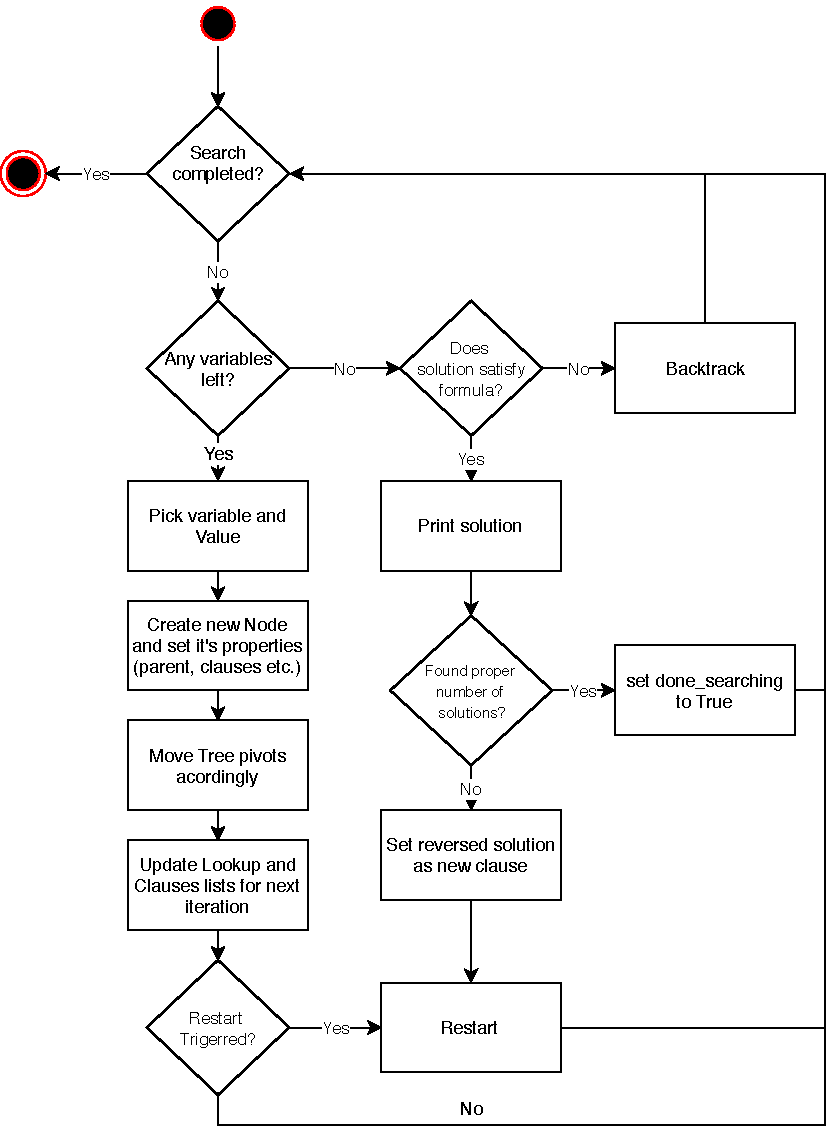
\includegraphics[scale=0.9]{img/main_loop}
\par\end{centering}
\caption{Main loop high level flowchart}
\end{figure}

Of course many of the steps depicted with single blocks  are in fact quite complex procedures. Also,
due to non-chronological backtracking and periodic restart done by
the solver, it is impossible to verify if the formula is UNSAT at this level,
so UNSAT checks are done several times during individual function
calls. It is possible mostly because of the fact, that if the  formula is found to be UNSAT,
the entire solver can be shut down as there is nothing left to do.

The individual steps, represented as in-class functions of the class Tree
will be presented in the following flowcharts for better understanding
of the high-level design of the solver. For low level implementation, code inspection
can be performed.

Picking a variable and its value step is performed according to the following flowchart:

\begin{figure}[H]
\begin{centering}
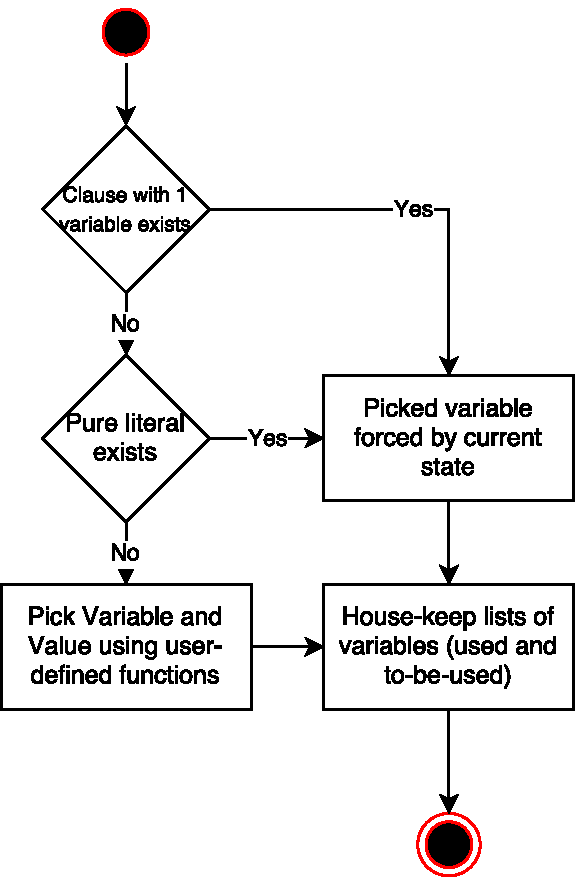
\includegraphics[scale=0.7]{img/pick_var_and_val}
\par\end{centering}
\caption{Value and Variable decision flowchart}
\end{figure}

As on a the figure above, replaceable functions for choosing value and variable
are not always used. They are only used whenever arbitrarily choice
has to be made. If any clause is found to be a unit one (it contains only one literal), 
the proper variable is
picked and its value is assigned so that the clause is satisfied. Also, if there is any pure
literal within the formula, it also can be safely chosen and its value can be assigned before any further 
decisions are made.

After picking a variable and its value, an update of clauses and lookup
lists have to be made for the next iteration -- Unit propagation(\ref{subsec:UnitProp}) is being applied on the current state of clause lists. The
only pitfall that might happen is that the variable was left in two different
clauses as the only literal -- but with different signs. When this
variable is  chosen and one of the values is be assigned to it,
a conflict will be detected while updating the second unit clause.

\begin{figure}[H]
\begin{centering}
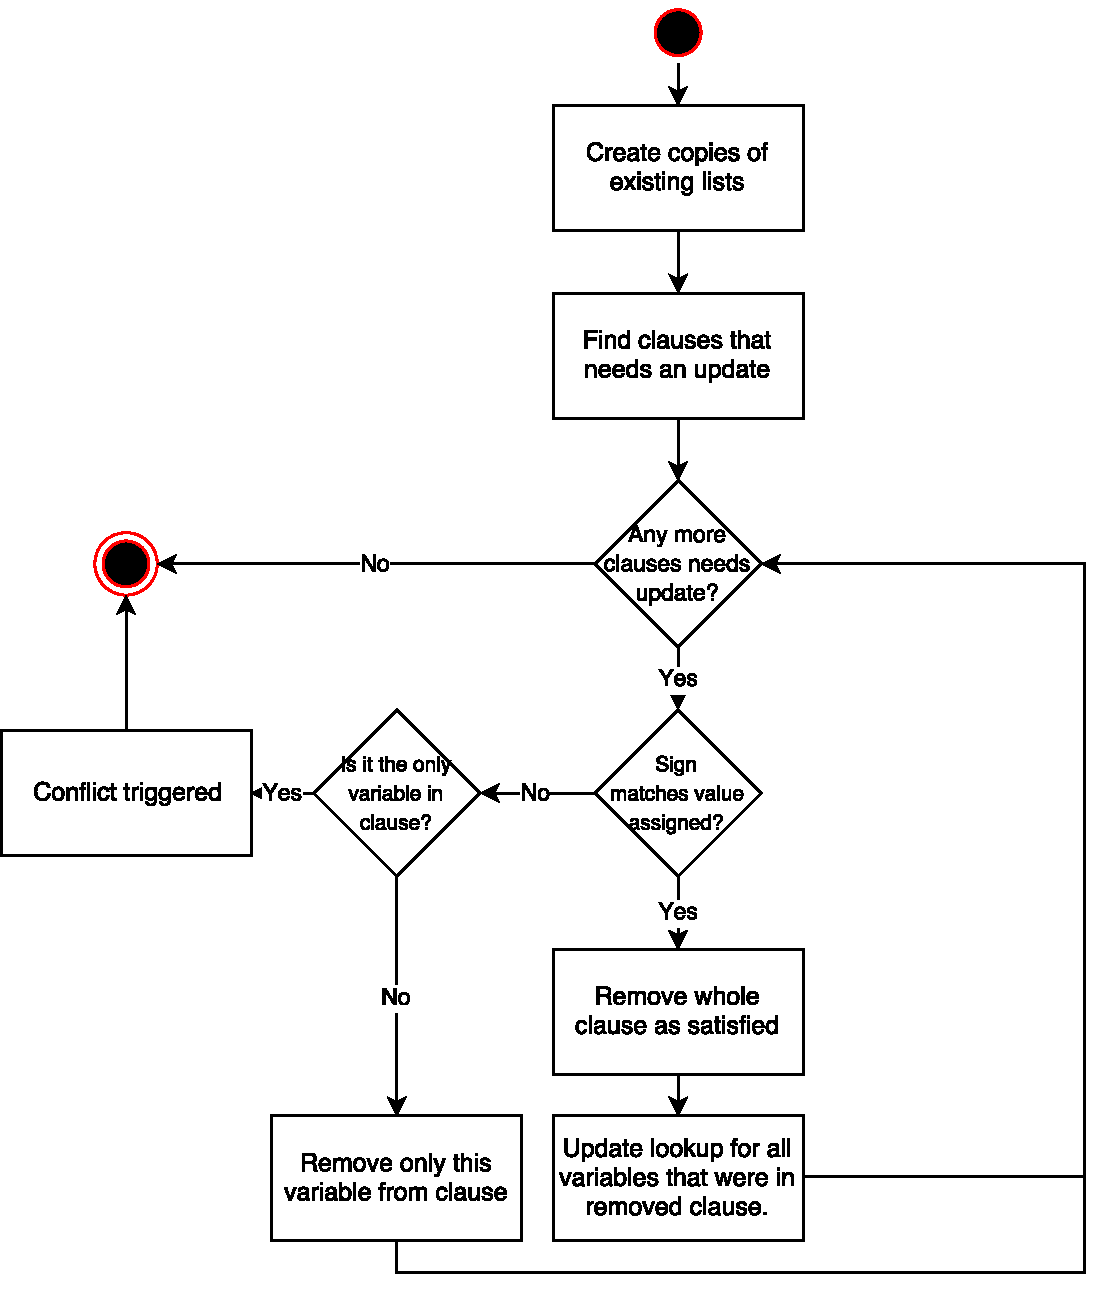
\includegraphics[scale=0.7]{img/update_variable}
\par\end{centering}
\caption{Clauses and Lookup lists updates.}
\end{figure}

The next step that needs to be defined within the solver is the action that will
be taken if a conflict was detected. The steps that are taken by the solver
developed in this thesis are as followed:

\begin{figure}[H]
\begin{centering}
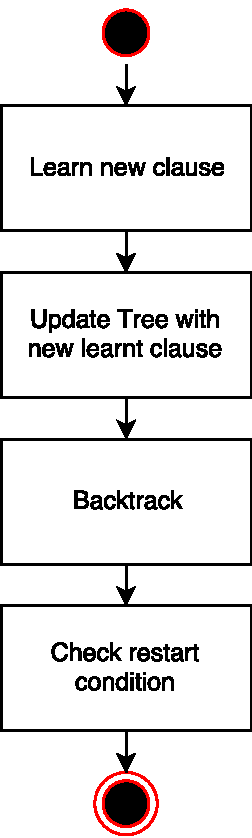
\includegraphics[scale=0.7]{img/conflict_detected}
\par\end{centering}
\caption{Conflict detection flow}
\end{figure}

The main still  remaining question is how to learn the clause and how to backtrack.
The following flowchart represents clause learning from code-based perspective.
Examples with detailed explanation of each step will be presented
afterwards.

\begin{figure}[H]
\begin{centering}
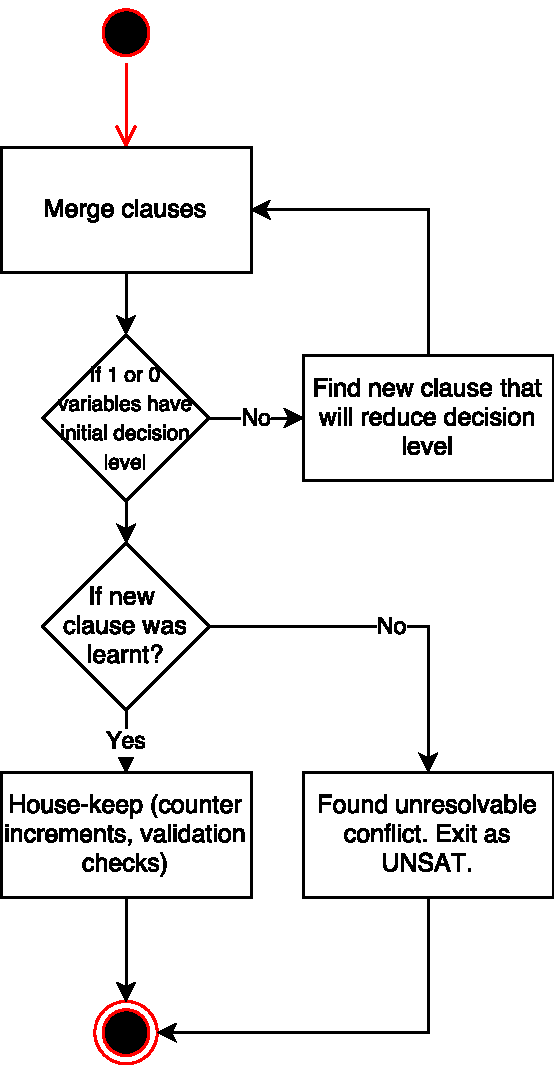
\includegraphics[scale=0.7]{img/learn_clause}
\par\end{centering}
\caption{Clause learning flow}
\end{figure}

When a new clause is learned by the solver, it needs to be propagated to
all nodes that are already present in the tree, so that it can be useful in
future search. It is especially important if backtracking was
not done chronologically. As the solver may leave some branches not fully
searched, and when it comes back to them, the new clause might become
useful.

\begin{figure}[H]
\begin{centering}
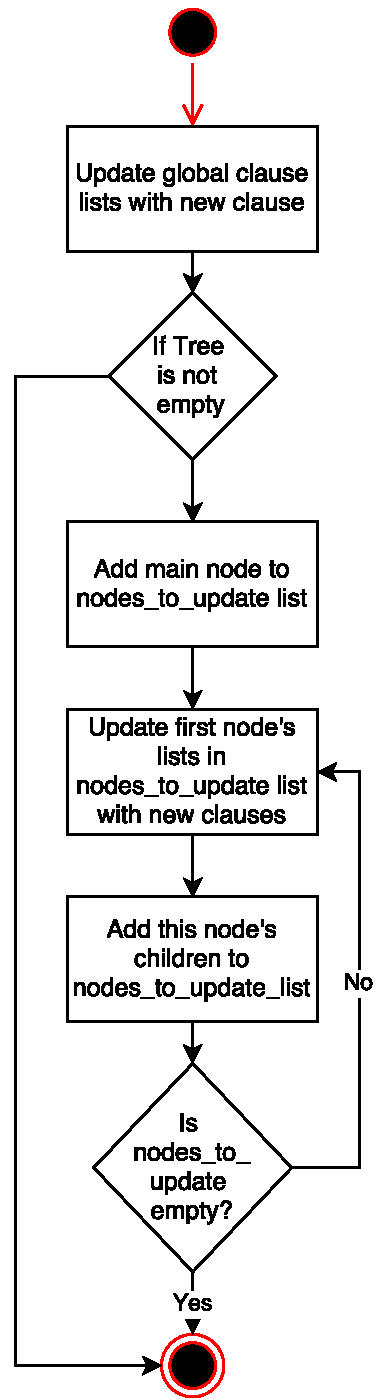
\includegraphics[scale=0.7]{img/update_tree_with_clause}
\par\end{centering}
\caption{Update tree with new clause}
\end{figure}

The remaining steps of conflict detection are based on replaceable function,
so their logic might differ depending on which function was used
within single run.

\section{Clause learning and non-chronological backtracking}

This chapter will present logical idea on two main breakthrough ideas
behind any CDCL based Solver. The main technique used to learn new clauses
and a function of non-chronological backtracking will be explained. 

The first steps look very similar
to those done in DPLL algorithms presented in Fig.~\ref{fig:DPLL}.
For better introduction to these algorithms, an example will be presented.
To make it more readable, decisions will not base on pure
literals, but only on unit clauses.

Consider the following example of SAT formula:

\begin{lstlisting}
p cnf 9 9
1  2                     0
1 -2  3  4               0
        -4  5            0
     -3     5            0
      3 -4    6 -7       0
             -6  7  8    0
        -4      -7 -8    0
                    8  9 0
                -7    -9 0
\end{lstlisting}
The first step to do is to choose  a Variable and its Value in an arbitrary way, and make
a unit propagation if possible. 

\begin{figure}[H]
\begin{centering}
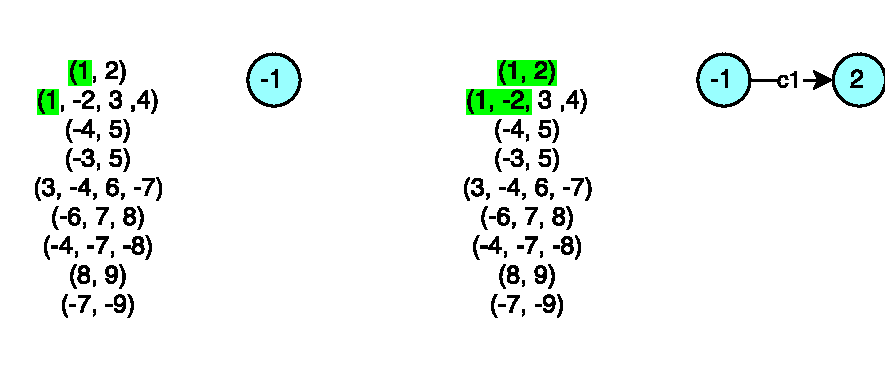
\includegraphics[scale=0.8]{img/CDCL_1}
\par\end{centering}
\caption{The first step of the CDCL algorithm}
\end{figure}

There are 3 important pieces of data that needs to be stored. The first and obvious one, 
is a list of clauses. After $x_1$ was assigned to $\mathsf{FALSE}$, the 1st
clause becomes a unit one,  which forces the solver to pick $x_2$ and assign $\mathsf{TRUE}$
value to it. 

The second important data to be stored, is a decision
level of each variable. Decision level is only increased if arbitrary
decision is done. If variable is \textit{forced} to be picked -- decision level
is equal to the decision level of latest arbitrarily chosen variable.
In this case both variables have the same decision level\footnote{The 1st decision level is marked as light blue color}. 

The last important information stored within each variable
that was \textit{forced} to be picked, is number of clause responsible for its assignment.
In this example, $x_2$ was assigned $\mathsf{TRUE}$ for the sake of satisfying the first clause.
So $x_2$ stores the information that clause number 1 was responsible
for its assignment.

When the entire unit propagation is done, the next variable is chosen in an arbitrary way.

\begin{figure}[H]
\begin{centering}
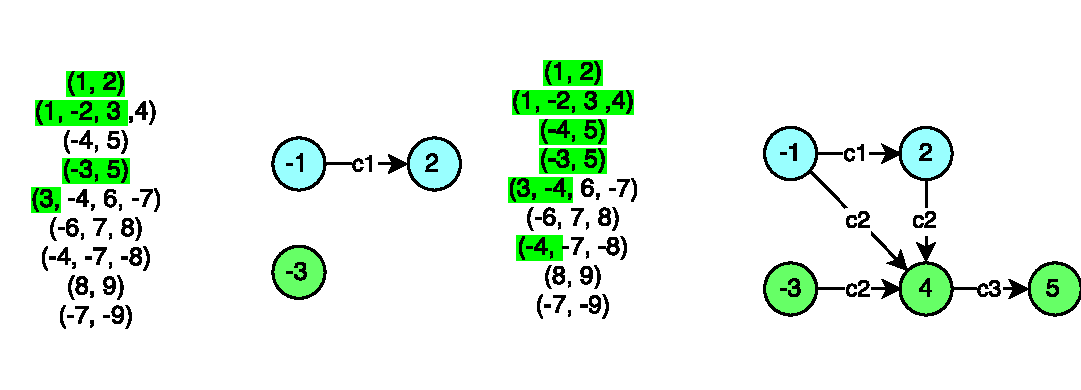
\includegraphics[scale=0.8]{img/CDCL_2}
\par\end{centering}
\caption{Second step of CDCL}
\end{figure}

The next variable picked was $x_3$ -- and the value assigned to it was
$\mathsf{FALSE}$. Next,  $x_4$ and $x_5$ were picked, due to clauses number 2 and ,3 respectively.
Moreover, an important note is that a decision level of those variables raised
to 2\footnote{decision level 2 noted as light green color on graph}.

\begin{figure}[H]
\begin{centering}
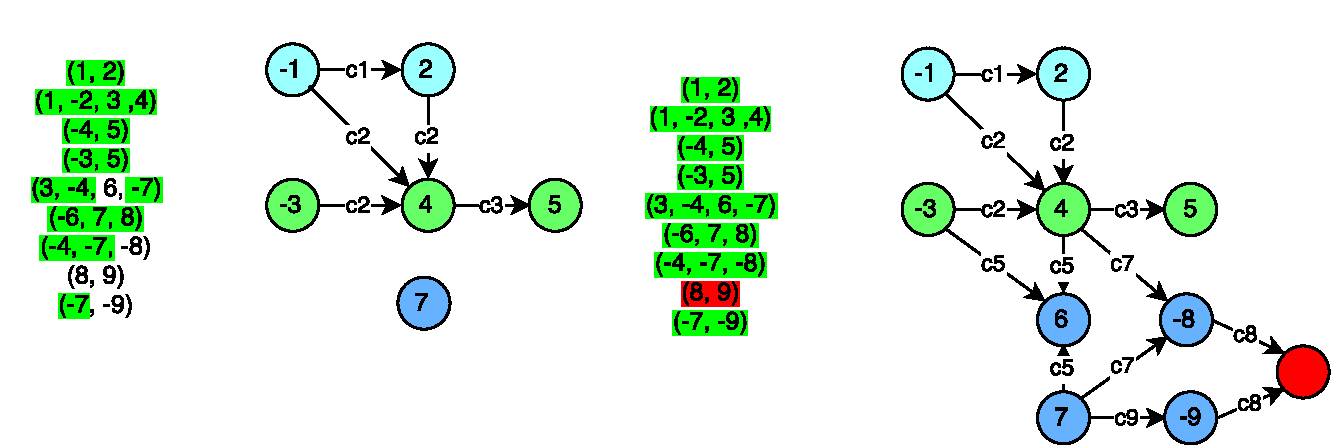
\includegraphics[scale=0.7]{img/CDCL_3}
\par\end{centering}
\caption{Third step of CDCL}
\end{figure}

Once again, another level of decision was created\footnote{decision level 3 noted as darker blue on graph}.
Variable $x_7$ was picked with $\mathsf{TRUE}$ value, and the rest of variables were
forced to be assigned. While one of the unit propagation procedures, the solver detects
that one of the clauses cannot be satisfied with those assignments; hence,
a conflict is detected.

What is most noticeable here, is that by now
the presented approach  does not really differ from the DPLL algorithm. As mentioned before,
only representation of data differs a little, and the information stored
are extended. It would not be much of a trouble to transform that form into
more DPLL-friendly form. The first real idea that differs those two algorithms
is the previously  mentioned \textit{clause learning}. There are of course many
different approaches to that problem, but this presented here was
implemented within the developed solver.

The main thing to remember is that any two clauses can be mixed together
into one clause. The remaining question is if the new learned clause will
be further useful or not. For this CDCL-based solver, the approach that
was taken will try to merge clauses as long as only one  variable within
this clause remains in the same decision level as the conflicted values.
Clauses that are merged are taken from the implication graph above. Merging
functionality is done using simple laws of Boolean algebra. It is explained
in more details in subsection \ref{subsec:Clause-evaluation}.

Clause merging showed on example presented above:
\begin{figure}[H]
\begin{centering}
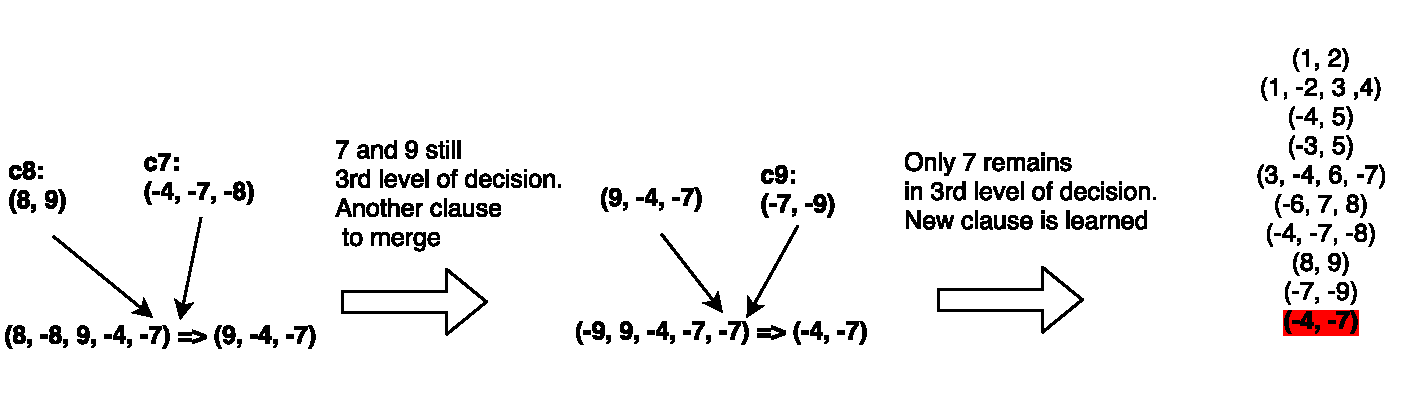
\includegraphics[scale=0.6]{img/CDCL_learning}
\par\end{centering}
\caption{Learning new clause by merging}
\end{figure}
The same example using implication graphs is presented below.\footnote{Clause merging is actually a special way of using Propositional Resolution (\ref{sec:resolution}), in such a way that an expected result is achieved.}:

\begin{figure}[H]
\begin{centering}
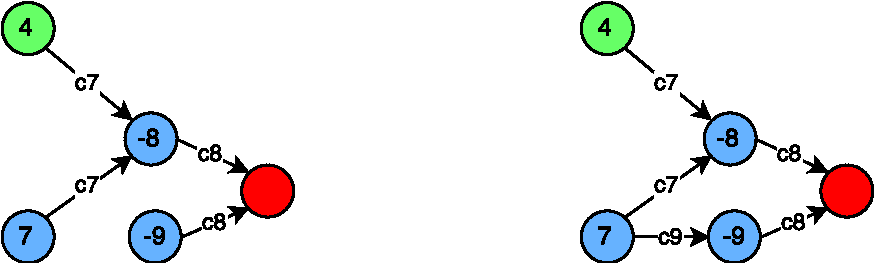
\includegraphics[scale=0.7]{img/CDCL_implgraph}
\par\end{centering}
\caption{Learning new clause with graph structure}
\end{figure}

When a new clause is learned, it is added into the database. It also has
to be propagated to all existing nodes within the tree as each node keeps
their own version of clause database. 

At this point backtracking technique needs to be applied. Traditionally, SAT
solvers use \textit{chronological backtracking} described in previous chapters.
However, to make most of the newly learned clause, \textit{non-chronological backtracking}
is used. Again, as with clause learning -- every solver can implement
its own individual algorithm, and the one described here is the one
that was used within the presented implementation. The idea is to backtrack to the
second highest decision level present in the newly learned clause. So
in the given example, $x_4$ has decision level of 2 and $x_7$ has
decision level of 3. The 2nd highest decision level in this case is
2\footnote{it is possible that a newly learned
clause contains only 1 variable. Its decision level would be 0 -- it is the decision level for all variables that can be assigned before first arbitrary decision.}.

\begin{figure}[H]
\begin{centering}
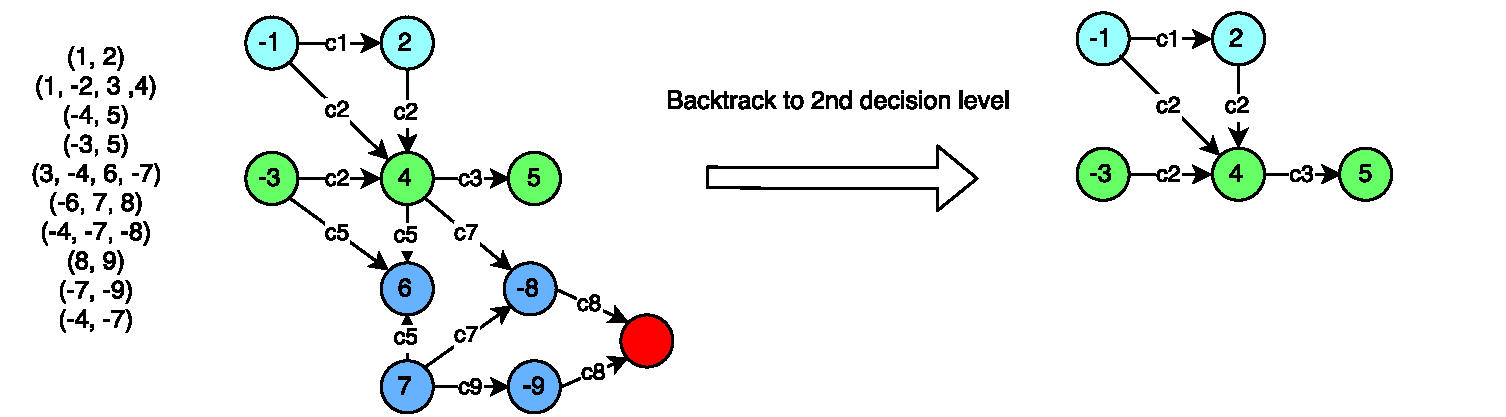
\includegraphics[scale=0.6]{img/CDCL_BT}
\par\end{centering}
\caption{Non-chronological backtracking}
\end{figure}

After  backtracking procedure is performed, again, a unit propagation procedure is applied.

\begin{figure}[H]
\begin{centering}
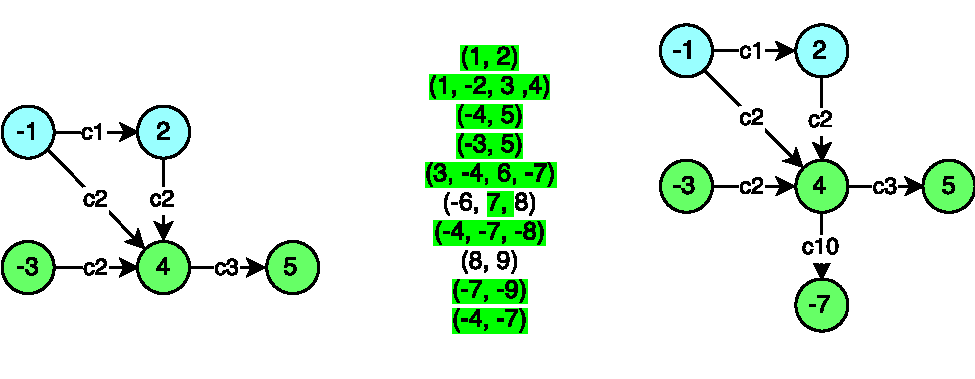
\includegraphics[scale=0.7]{img/CDCL_afterclauselearn}
\par\end{centering}
\caption{Unit propagation after backtracking}
\end{figure}

The only thing left to do is to make one more decision. However, it is trivial to prove
that whichever values are picked, the following formula will be satisfied. 

What can be clearly proven here, is that falling back to 2nd highest
decision level from the learned clause actually made a difference. It
allowed the solver to immediately make use of the newly learned clause. Also,
with deeper analyzes, the solver could notice that the newly created clause
is actually a sub-clause for clause number 7, thus clause number 7 could
be removed from the database (if clause $\neg x_4 \vee \neg x_7$ has to be satisfied, the wider
clause $\neg x_4 \vee \neg x_7\vee \neg x_8$ has to be satisfied as well).  

\section{Other Specialized Functions}
\label{sec:OtherFuncs}

Apart from 2 backtracking functions, which are shown on graphs
described in previous chapters, the rest of the specialized functions
are trivial. Restart functions are usually based on number of learned
clauses. They allow the  solver not to be restarted too rarely, or without
any progress with solving. An example of restart function is as follows:

\begin{lstlisting}
def restart_each_fifty(self):
    if self.number_of_learnt_clauses % 50 == 0 and self.number_of_learnt_clauses > 0:
        return True
    else:
        return False
\end{lstlisting}
Here the solver will get restarted every 50 clauses learned.

The Variable functions implemented are usually based on the number of occurrences
within formula, and differences in positive and negative occurrences.
Simple example of that function is given below.

\begin{lstlisting}
def choose_var_based_on_prob(self):
    if self.variables_to_use:
        var = max(self.variables_to_use, key=lambda x: abs(x.probability))
        return var
    else:
        return None
\end{lstlisting}
The sample function will return variable that has the highest occurrence probability
in initial formula. It is of course very trivial example as it does
not upgrade each learned clause or even each node created\footnote{probability member is calculated at input reading and it does not refresh while searching}.

With Value functions it gets even more simple then that. Since  having a
variable picked it is easy to define a function that determines what
value should be assigned to it. It can always return TRUE if possible,
or always return FALSE, or it can base the decision on occurrences of given
variable within all formulas. An example follows:
\begin{lstlisting}
    def return_based_on_prob_rev(self):
        var = self.latest_var.number
        lookup = self.next_iteration_lookup[var-1]
        positives = sum(1 for x in lookup if x > 0)
        negatives = len(lookup) - positives
        return positives > negatives
\end{lstlisting}
In this function, it is checked if a given variable occurs more frequently  as a positive
literal, or as a negative literal, and the value that reduces
more clauses is returned.




\chapter{Testing and Results}
\label{chap:Results}

\section{Testing Framework}
\label{sec:Framework}

Testing of the implemented SAT-solver was divided into 2 parts. First, a set of
tests was implemented to ensure that results of the SAT Solver were
correct, as this is the core requirement for any SAT Solver -- to provide
correct answers. The second set of tests was designed to observe behavior
of the SAT Solver on some collection of input formulas.

Functional tests for the correctness of output were not sophisticated.
The SAT  Solver was tested by variety of inputs (manually crafted, as well as
randomly generated). Then, the results were compared with results gathered
from other accessible SAT Solvers to ensure that outputs were matching. Both
satisfiable and unsatisfiable formulas were tested, and all encountered
bugs were fixed (to match main requirement of every SAT Solver). 

An important
note here is that within satisfiable formulas, only formulas with exactly
one result could be automatically tested. That is because both solvers
could come up with correct solution, but with a different one. It could
lead to the detection of false negative examples. Results of those tests
will not be presented  because of their simplicity.

For behavioral testing, an external script was developed. This script
allows to launch the SAT Solver on every DIMACS format file within
a given directory. It also measures the time of solving for each file separately
and for all of them together. The testing script can be launched with the exactly
same user options as the SAT Solver itself and those options will be passed to the solver.

\section{Tested Inputs}
\label{sec:testinputs}

The main issue with selecting proper inputs for testing purposes
is to balance the number of clauses with the number of variables.  
Without proper
clauses-to-variables ratio, satisfiability problem might be either
trivially SAT (with too much variables) or trivially UNSAT (with
too much clauses).

As input examples for testing, randomly generated DIMACS formulas were used.
In particular, all used formulas are 3-SAT (Each clauses consists
of exactly 3 literals). Strict 3-SAT formulas were chosen to keep the ratios consequential\footnote{Without strictly set K-SAT formulas, results would highly depend on size of clauses within formula. This allows results to be proportional to the size of the input formula}. Clauses were generated by ThoughSat
application \cite{ToughSAT}. The main goal of this testing, was to observe
the maximum capability of implemented solver as well as to compare different settings.

To observe maximum capacity of the implemented solver with different inputs,
some groups of inputs were distinguished, based on clauses-to-variable
ratio:
\begin{itemize}
\item Main group of formulas -- \textit{Tough formulas} -- where the ratio oscillates
between 3.5 and 5 (with toughest problems being between 4.2 and 4.8); 
\item \textit{Trivially UNSAT} formulas -- where the ratio is higher then 5;
\item \textit{Trivially sat formulas} -- where ratio is lower then 3.5.
\end{itemize}
These ratios are based on observations of the solver behavior on variety of problems being
resolved by implemented it, as well as the behavior of some external solvers for
3-SAT formulas. For other SAT formulas, those ratios will be different.
For example for 4-SAT ones, the toughest ratios are oscillating somewhere near 10.

\section{Results}
As mentioned previously, the solver passed all of the predefined tests for correctness -- no invalid output were found. So the results of the solver (outputs of the solver) are not the thing under testing here. The following results will contain a set of comparisons concerning  time consumption of the solver with different settings on various inputs.

To make the results more comparable, some sets of setting were assumed:
\begin{enumerate}
\item Intuitively the best possible setting:
\begin{itemize}
\item Variable is chosen based on probability,
\item Value is chosen to satisfy as much clauses as possible,
\item Non-chronological backtracking based on learnt clause is used,
\item Restart condition increased by 20 learnt clauses each time, starting from 30.
\end{itemize}
Arguments passed:
\begin{lstlisting}
--var=A --val=A --backtrack=C --restart=S
\end{lstlisting}

\item Naive CDCLalgorithm  without variable deductions:
\begin{itemize}
\item Variable chosen without any algorithm,
\item True value is returned if possible,
\item Non-chronological backtracking based on learnt clause is used,
\item Restart each 50 clauses learnt.
\end{itemize}
Arguments passed:
\begin{lstlisting}
--var=N --val=T --backtrack=C --restart=F
\end{lstlisting}

\item Smart DPLL with restarts introduced
\begin{itemize}
\item Variable is chosen based on probability
\item Value is chosen to satisfy as much clauses as possible
\item Chronological backtracking
\item Restart condition multiplied by 2 each time, starting from 10.
\end{itemize}
Arguments passed:
\begin{lstlisting}
--var=A --val=A --backtrack=P --restart=M
\end{lstlisting}

\item Naive DPLL algorithm with restarts introduced:
\begin{itemize}
\item Variable chosen without any algorithm,
\item True value is returned if possible,
\item Chronological backtracking,
\item Restart each 50 clauses learnt.
\end{itemize}
Arguments passed:
\begin{lstlisting}
--var=N --val=T --backtrack=P --restart=F
\end{lstlisting}

\item Experimental variable mixture:
\begin{itemize}
\item Variable with most positive literals chosen,
\item False value returned if possible,
\item Non-chronological backtracking based on learnt clause,
\item Restart each 50 clauses learnt.
\end{itemize}
Arguments passed:
\begin{lstlisting}
--var=H --val=F --backtrack=C --restart=F
\end{lstlisting}

\end{enumerate}

Those settings will be tested on inputs described in more details in Section~\ref{sec:testinputs}. To achieve better results, each set of inputs will contain 10 equally large formulas to be solved. The results will present a summary time to solve each of those sets\footnote{To  get an average time for one formula, the given time can be simply divided by 10}. To prevent locking the CPU on some formulas, a timeout condition was introduced. Timeout is defined as solving a single formula for more then 2 minutes straight.

All tests were ran on a computer with following parameters:
\begin{itemize}
\item CPU: Intel® Core™ i5-3210M CPU @ 2.50GHz × 4,
\item Memory: 7,6 GiB,
\item OS: Ubuntu 16.04 LTS, 64-bits.
\end{itemize}

\subsection{Trivially SAT}
\label{subsec:TrivialSat}
Trivially satisfiable formulas are formulas with so little constraints that they will always\footnote{\textit{Always} here means -- \textit{very, very} likely from probability point of view} be satisfiable. As mentioned in Section~\ref{sec:testinputs} for strictly 3-SAT, such formulas could be defined with dependency: $\frac{No.\ of\ clauses}{No.\ of\ variables} \le 3.5$
The results for Trivially SAT formulas look as follow:
\begin{figure}[H]
\begin{centering}
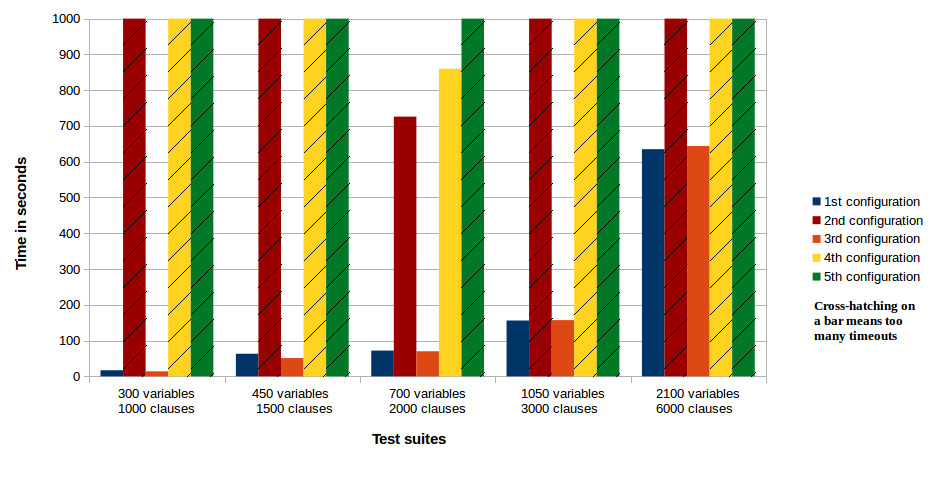
\includegraphics[scale=0.62]{charts/trivial_sat}
\par\end{centering}
\caption{Results of Trivially SAT formulas}
\label{fig:trsat}
\end{figure}
Results presented on Figure~\ref{fig:trsat} show that only the 1st and the 3rd configurations were able to solve even the simplest proposed formulas within given time of 2 minutes. The only exception is the 3rd test-suite with 700 variables and 2000 clauses. What causes this, is that in the 3rd test suite, the ratio is the lowest from all formulas, with $\frac{No.\ of\ clauses}{No.\ of\ variables} \approx 2,86$. Even though the 2nd and the 4th configuration were able to solve it within the given time limit, they are still much slower then configuration 1 and 3.

What stands out for the most successful configurations here -- the 1st and the 3rd -- is that their decision for value and variable are actually based on the current state of the search tree. This is the factor that makes them much faster then other configurations. Also, seeing the tendency of time growth on Figure~\ref{fig:trsat}, the maximum limit of clauses is near 3000 with time limit set to 2 minutes.

\subsection{Tough SAT}
\label{subsec:ToughSat}
Tough formulas are the main concern for every solver. They are the most difficult and challenging to solve. As mentioned in Section~\ref{sec:testinputs}, difficulty of a formula depends on the clause-to-variable ratio, as well as the number of literals within a clause. The first set of results for difficult formulas is as follows:

\begin{figure}[H]
\begin{centering}
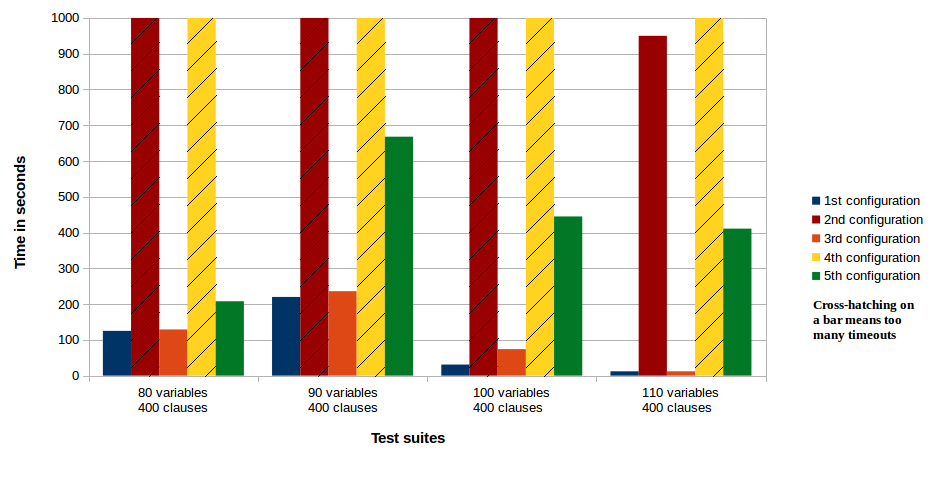
\includegraphics[scale=0.62]{charts/diff_sat_1}
\par\end{centering}
\caption{First set of results for tough formulas}
\label{fig:diffsat1}
\end{figure}

Results presented in Figure~\ref{fig:diffsat1}, again show that configuration 2 and 4 are practically useless. They will be purged for the rest of those results, as formulas will only become tougher.

This chart shows also an advantage of non-chronological backtracking, as on average it is more efficient in solving those problems. The 5th configuration was able to solve many of given problems in decent time, however the timing was much more unstable then the 1st and the 3rd configurations. Some of more difficult problems were solved by it almost immediately, whereas sometimes it would get the timeout on simpler instances. The next chart will present those successful configurations against formulas with the same ratio as before, but bigger in numbers:

\begin{figure}[H]
\begin{centering}
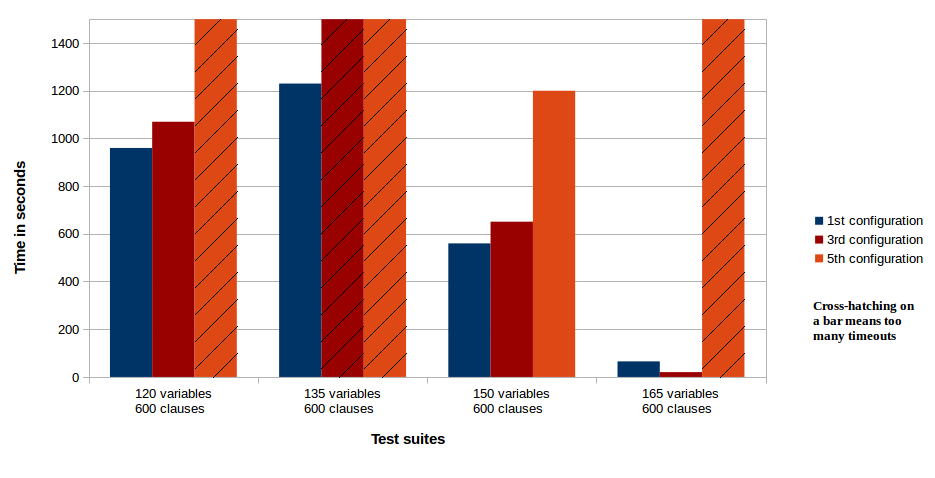
\includegraphics[scale=0.62]{charts/diff_sat_2}
\par\end{centering}
\caption{Second set of results for tough formulas}
\label{fig:diffsat2}
\end{figure}

In formulas present in tests showed in Chart~\ref{fig:diffsat2}, \textit{luckiness} of configuration 5 becomes a less significant factor. That caused the timeout on almost all instances of tested inputs. 

Non-chronological backtracking remains a bit faster then chronological backtracking. The difference remains similar to the one in Chart~\ref{fig:diffsat1}. Also, as all configurations  closely approached the timeout of 2 minutes, in the next experiments the timeout was  extended to 6 minutes per formula, and test suites will be reduced to 5 input files per suite. The results look as follow:

\begin{figure}[H]
\begin{centering}
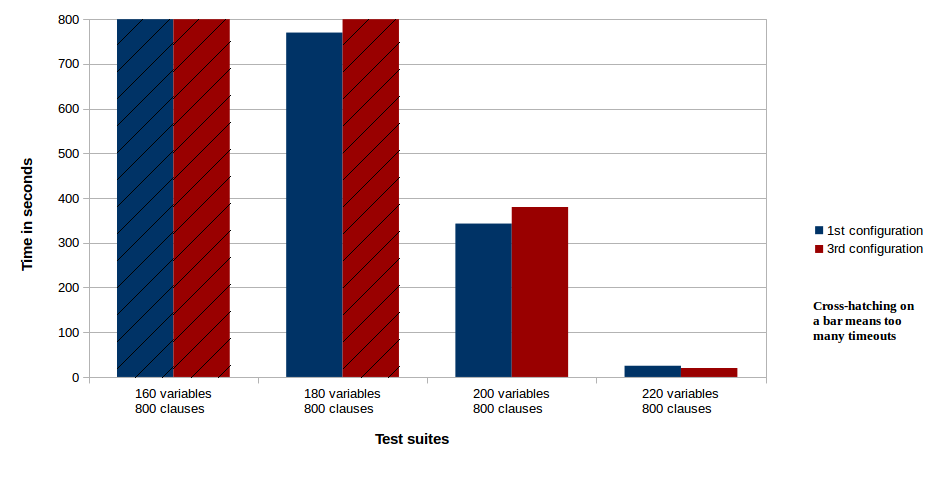
\includegraphics[scale=0.62]{charts/diff_sat_3}
\par\end{centering}
\caption{Third set of results for tough formulas}
\label{fig:diffsat3}
\end{figure}

Results shown in Chart~\ref{fig:diffsat3}, visualize that both configurations start to timeout in the most difficult ratio -- $\frac{No.\ of\ clauses}{No.\ of\ variables} \approx 4.5$. That shows the maximum potential for the implemented solver given the toughest possible formulas.

\subsection{Trivially UNSAT}
\label{subsec:TrivialUnsat}
Trivially UNSAT formulas are formulas with so much constrains that, in theory, it would be easier to find inconsistencies that prove unsatisfiability. However, as the implemented solver has a mechanism to find such inconsistencies, it struggles with UNSAT formulas as it has to pretty much decline all possible models. It causes the UNSAT formulas to explode in time very fast. With even minor increase in variables, time consumption grows inappropriately faster. The results for UNSAT formulas look as follow:

\begin{figure}[H]
\begin{centering}
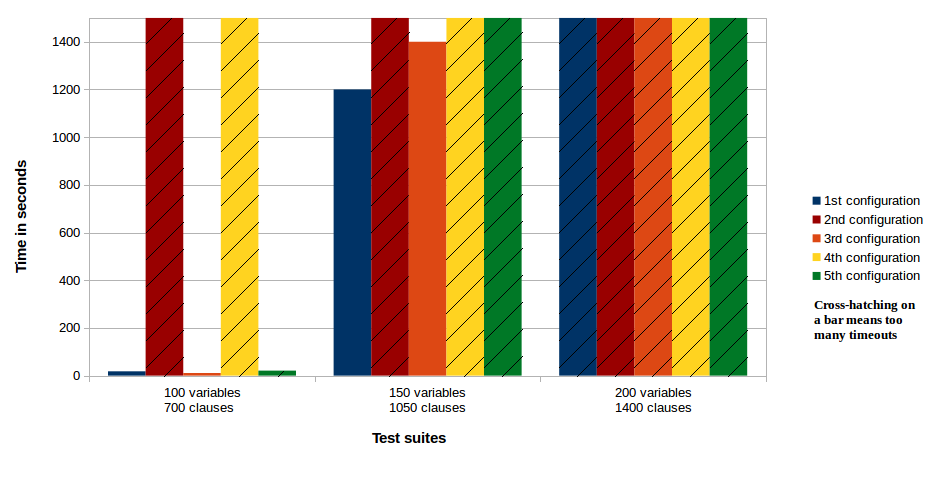
\includegraphics[scale=0.62]{charts/trivial_unsat}
\par\end{centering}
\caption{Results for trivial UNSAT formulas}
\label{fig:trvunsat}
\end{figure}
Figure~\ref{fig:trvunsat} presents that for 100 variables, formulas are solved almost immediately. However, adding 50 more variables (and clauses proportionally), causes almost every formula to timeout with no  solution found. That shows how it is difficult to define a proper testing inputs for solvers, as even small change in parameters might influence final outcome.

\chapter{Conclusions}
\label{chap:Conclusions}

\section{Outcome of the project}
This thesis began with a theoretical analysis of logic, in particular propositional calculus, and resolution. Those topics are the background of the satisfiability problem, and they are described in Chapter~\ref{chap:logic} with explanations and examples.

Further research of background of satisfiability problem, led to analysis of current state of SAT solvers with some technical details and standardization. Every aspect of that background is described in details in Chapter~\ref{chap:SoA-2}.

For further implementation, a deep understanding of some basic heuristics is needed. Those are described in Chapter~\ref{chap:Heuristics}. In this Chapter it is shown how to start implementation and how to approach solving satisfiability problems. Deep explanation of some algorithms described here could help to implement a SAT solver in every programming language from  scratch.

The implemented SAT solver consists of over 1000 lines of code written in Python. It implements many of the heuristics described in Chapter~\ref{chap:Heuristics}. From the high level design perspective, the code is described in Chapter~\ref{chap:Impl-4}. This Chapter also contains details about implementation of programming interface which could allow further development, as well as the user interface. As the implemented solver is based on the Conflict-Driven-Clause-Learning, details of this algorithm can be also found in here.

Results from Chapter~\ref{chap:Results} are illustrating and measuring the capabilities of the implemented Solver. They also show the difference between configurations of it, as well as the importance of each implemented functionality. 

In conclusion, the main goal of the thesis was accomplished, as the SAT-solver with open architecture was implemented. However there are 2 main issues that have to be raised. Firstly, SAT-solver is a program that never reaches its final state. SAT-solvers can vary from a simple brute-force program in few lines of code, to modern high-tech solvers that are unbelievably efficient. So there is always a room for improvements. Also, with such possibilities of input formulas, it is impossible to verify every possible corner scenario. So the correctness of outputs for the solver was tested to the best of the acceptable time and available resources. 

The second issue that is of interest, is the efficiency of implemented solver. One of the goals of this thesis, was to compare the implemented solver with some of the popular ones. However, those sat-solvers are being developed for years by groups of scientists, who were able to push those solvers to their limits. The efficiency of the implemented SAT-solver is nowhere close to those professional ones, so comparing them at this state presents no useful information. The solver implemented as a part of this thesis could be considered as a good, generic prototype that can be a base for further improvements and development an obviously for diversified experimental work.

\section{The Future of the project}
The code base for this project, as well as all tools used while writing it and test suites used for testing will be published on-line under GNU public license.

In the future, the first thing that will be done is assurance that this is compatible with Python 3.5. Also the work will have to be done to ensure compatibility with future Python releases. The source code will remain maintained and all found bugs will be addressed.

As SAT-Solvers are continuously developed, it is impossible to define an \textit{end state} of such program -- there is always a room for improvements. With given state, most of improvements are connected with lowering memory usage and time optimization. Hopefully, this project will gather some active contributors, who would help with improving the efficiency and memory management, as well as create new and interesting features (For example, those briefly mentioned in section~\ref{subsec:ModernCDCL}.

\section{Manual}
By the time this thesis is published, the whole source code will be available on-line at \url{https://github.com/bastior/masterThesis}. To launch the solver, one needs to execute \textit{code/aghSolver.py}, placed in \textit{code} directory, with Python 3 interpreter\footnote{As mentioned in chapter \ref{chap:Impl-4}, only Python version 3.6.1 was verified. There is no guarantee that any other version will provide correct output. In the future the support for Python version 3.X might be provided.}, with the input file given as argument:
\begin{lstlisting}
$ python3 aghSolver.py ../simpleTests/myth.cnf
\end{lstlisting}
Other arguments can be used to tune solver with customized settings:
\begin{lstlisting}
$ python3 aghSolver.py ../simpleTests/myth.cnf --var=A --val=A --backtrack=P --restart=M
\end{lstlisting}
More precise tutorial will be published with source code in on-line repository.
 
Due to the limited usage of packages, no external modules should be required. Input arguments are described in this thesis in section \ref{sec:UI}. To run the solver on all \textit{.dimacs} and \textit{.cnf} files in directory, start Tests/testOnDirectory.py python script\footnote{Same User Interface parameters can be passed to it.}. Outputs will appear in the \textit{Results} sub-directory. Some examples of input formulas are available at the \textit{simpleTests} directory\footnote{simple dimacs formulas}, or the \textit{testFolders} directory\footnote{More complicated, randomly generated DIMACS formulas used for testing}. Any bugs or suggestions might be posted on the same page where the source code can be found.


\bibliographystyle{plain} % styl mozna zmienic
%%% Tu ponizej: wybor plikow z wykazami bibliografi typu .bib
\bibliography{%
bib/myBib%
}%
\end{document}
\grid
\grid
\grid
